\documentclass[11pt]{beamer}
\usetheme{Antibes}
\usepackage[utf8]{inputenc}
\usepackage[german]{babel}
\usepackage[T1]{fontenc}
\usepackage{amsmath}
\usepackage{amsfonts}
\usepackage{amssymb}
\usepackage{graphicx}
\author{Gruppe C14 \\ \textbf{Julián Häck}, Martin Koytek, Lars Wenning, Erik Zimmermann}
\title{Akustik}
\usepackage{multicol}
\usepackage{float}
\setbeamertemplate{footline}[frame number]
%\setbeamercovered{transparent} 
%\setbeamertemplate{navigation symbols}{} 
%\logo{} 
%\institute{} 
%\date{} 
%\subject{} 
\begin{document}

\begin{frame}
\titlepage
\end{frame}

\begin{frame}
\begin{itemize}
\item Schallgeschwindigkeit in Luft
\begin{itemize}
\item Variation der Frequenz
\item Vermessung der stehenden Welle
\item Laufzeitmessung
\end{itemize}
\item Schallgeschwindigkeit in Festkörpern
\item Versuche zur Gitarre
\begin{itemize}
\item Stimmen durch Schwebung
\item Materialeigenschaften
\item Frequenzspektrum
\end{itemize}
\end{itemize}
\end{frame}

\section{Bestimmung der Schallgeschwindigkeit durch Laufzeitmessung}
\subsection{Versuchsbeschreibung}
\begin{frame}{Bestimmung der Schallgeschwindigkeit durch Laufzeitmessung}
\begin{itemize}
\item Bestimmung der Schallgeschwindigkeit in Luft:
\begin{equation*}
v=\frac{s}{t}
\end{equation*}
\item Für die Temperaturabhängigkeit gilt:
\begin{equation*}
v=v_0\cdot \sqrt{\frac{T}{T_0}} 
\end{equation*}
\end{itemize} 
\end{frame}
\subsection{Versuchsaufbau und Durchführung}
\begin{frame}
\begin{figure}[H]
\centering
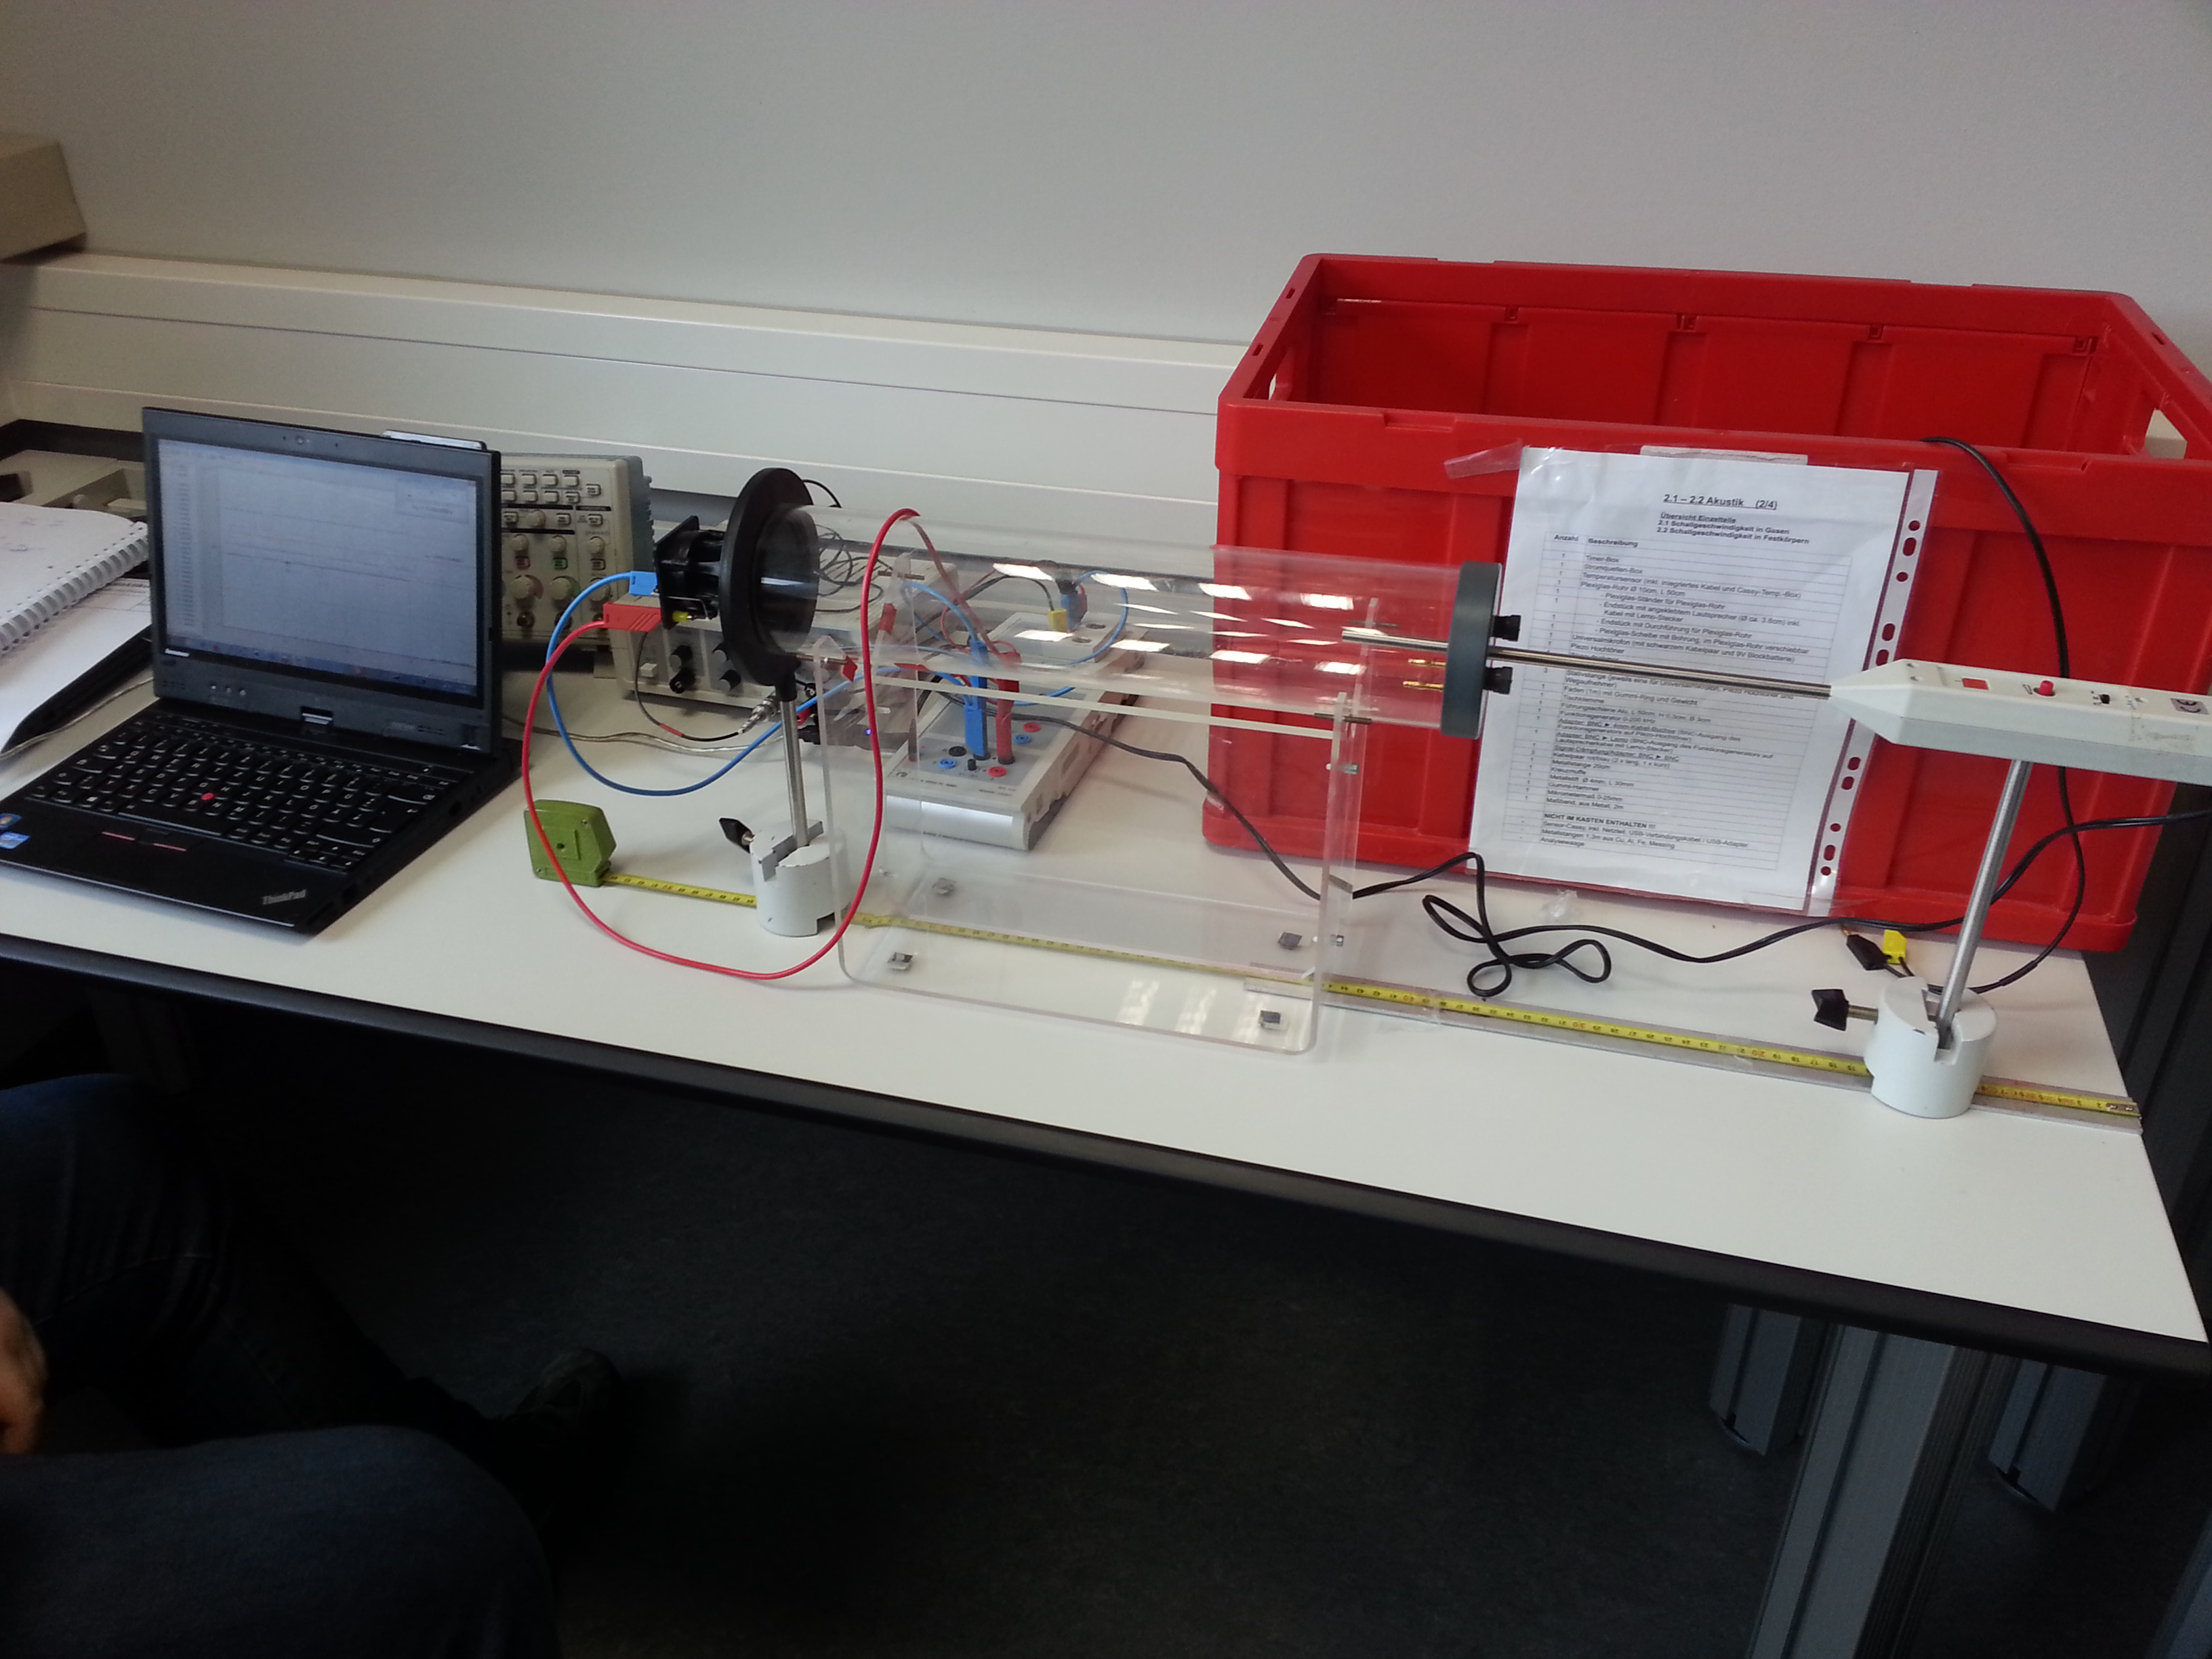
\includegraphics[scale=0.08]{Bilder/laufzeit-cassy.jpg}
\end{figure}
\end{frame}
\subsection{Rohdaten}
\begin{frame}
\begin{figure}[H]
\centering
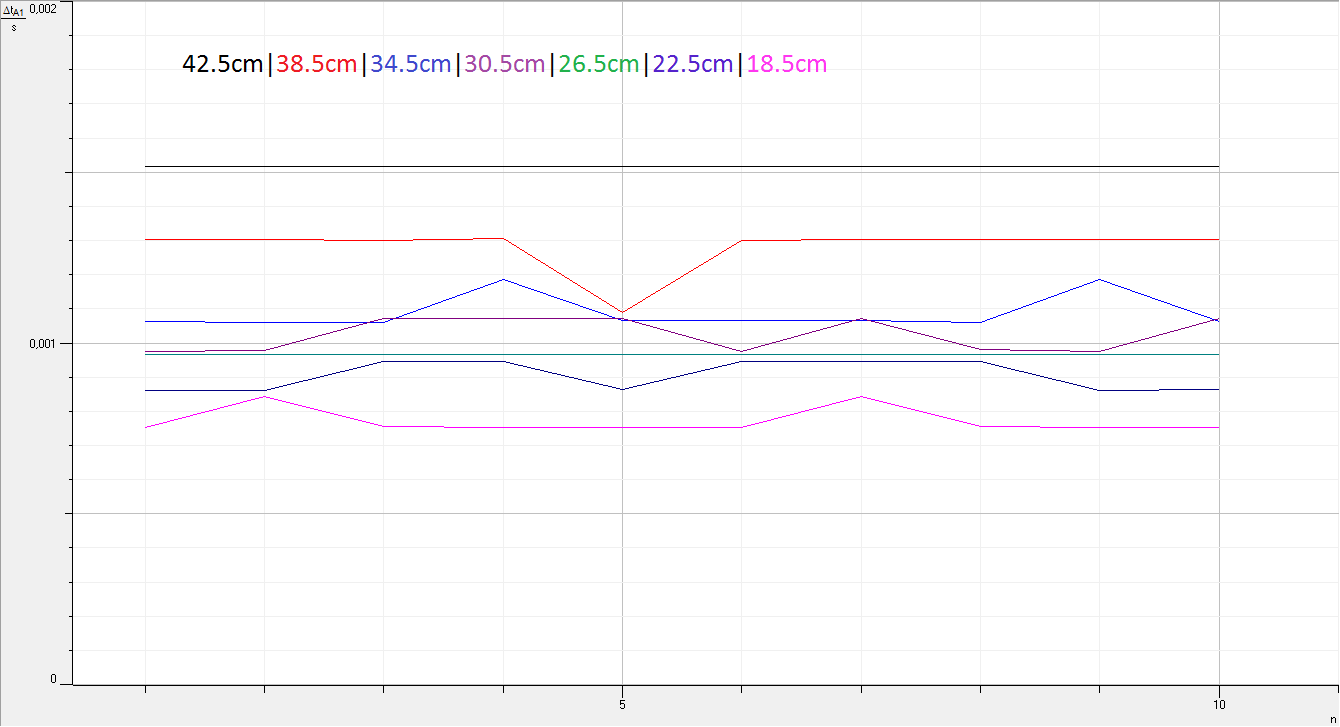
\includegraphics[scale=0.4]{Bilder/Rohdaten-Laufzeitmessung.png}
\label{Laufzeitrohdaten}
\end{figure}
\end{frame}
\begin{frame}
\begin{figure}[H]
\centering
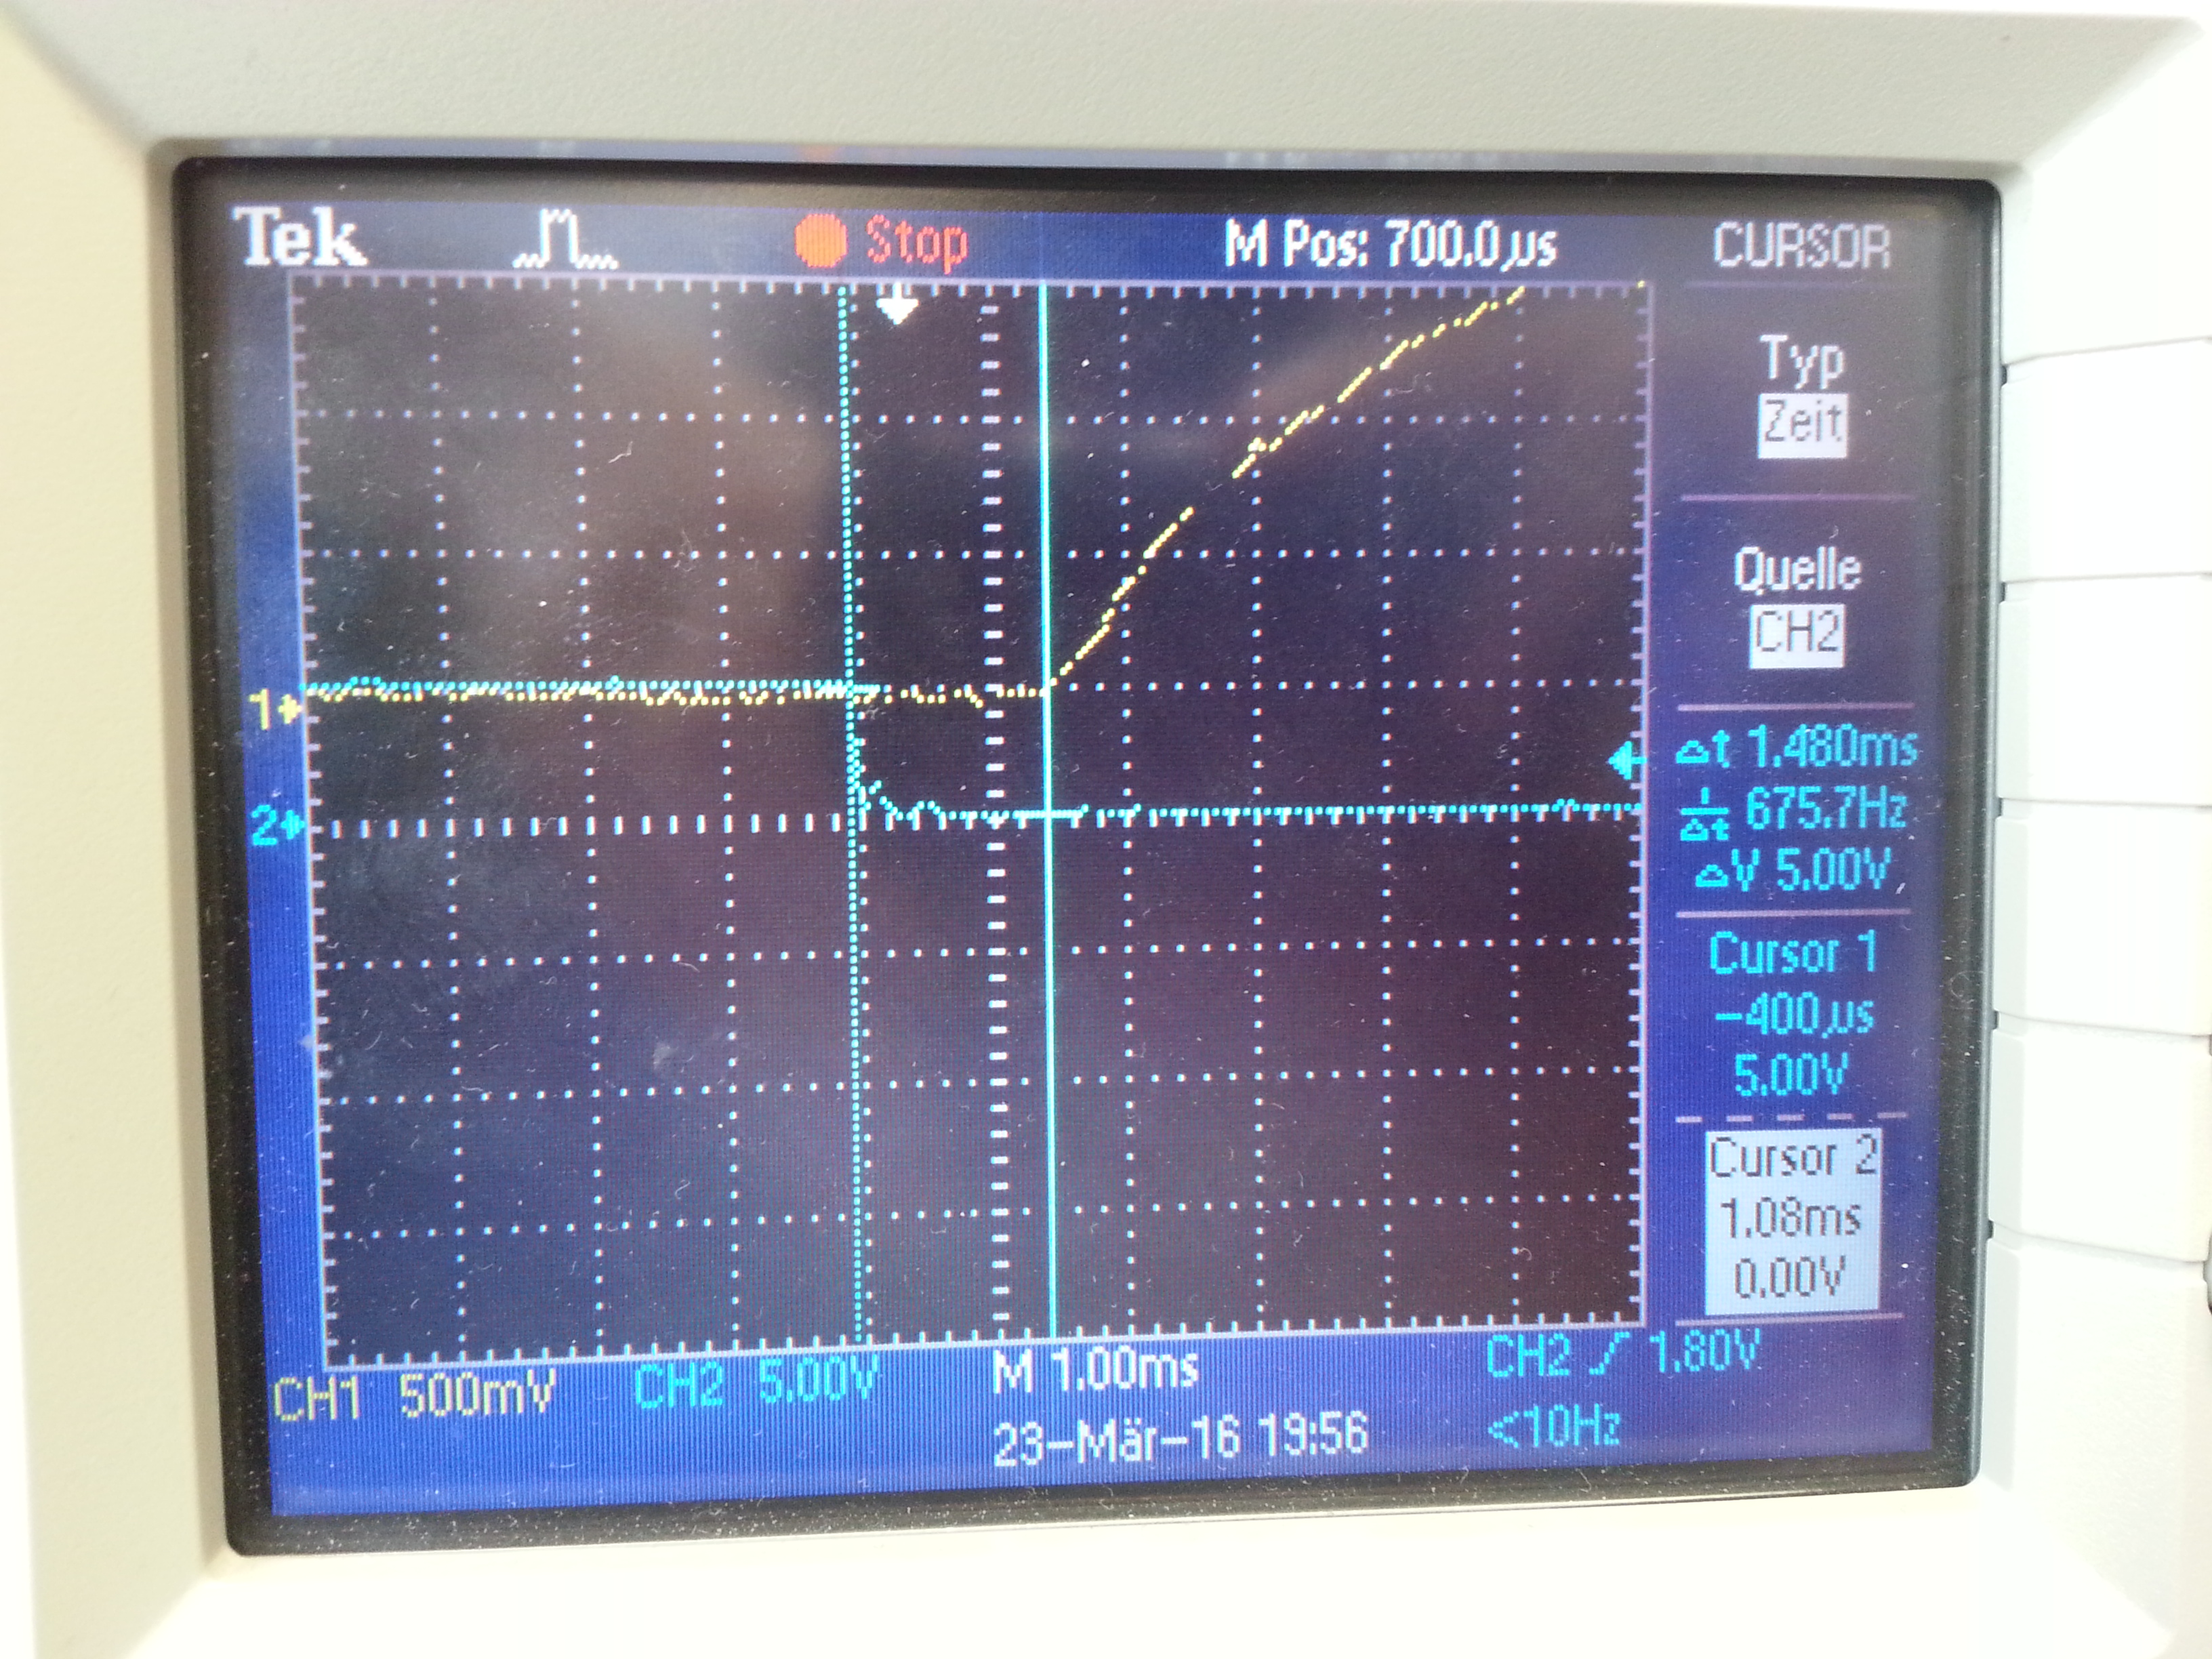
\includegraphics[scale=0.08]{Bilder/oszi.jpg}
\caption{L = 42.5cm}
\end{figure}
\end{frame}
\begin{frame}
\begin{table}[H]\centering
\caption{Werte der Laufzeitmessung mit dem Oszilloskop}
\begin{tabular}{c|c}
Abstand in cm & Zeitdifferenz der Spannungspeaks in ms\\ 
\hline
$42.5$& $1.48$\\ 
$34.5$& $1.24$\\
$26.5$& $1.08$\\
\end{tabular} 
\end{table}
\begin{itemize}
\item $\sigma_t=0.04ms$
\item $T=22.6^{\circ}C$
\end{itemize}
\end{frame}
\subsection{Transformation der Rohdaten/Analyse}
\begin{frame}
\begin{table}[H]\centering
\caption{Mittelwerte der Cassy-Laufzeitmessung mit Fehlern}
\begin{tabular}{c|c|c}
Abstand in cm & Mittelwert der Zeit in ms & $\sigma_t$ in ms\\ 
\hline
$42.5$& $1.51705$& $4.104 \cdot 10^{-4}$\\ 
$38.5$& $1.28692$& $7.141 \cdot 10^{-2}$\\
$34.5$& $1.08284$& $4.526 \cdot 10^{-2}$\\
$30.5$& $1.05089$& $4.390 \cdot 10^{-2}$\\
$26.5$& $0.96639$& $5.193 \cdot 10^{-4}$\\
$22.5$& $0.92490$& $3.756 \cdot 10^{-2}$\\
$18.5$& $0.80627$& $4.416 \cdot 10^{-2}$\\
\end{tabular} 
\end{table}
\end{frame}
\begin{frame}
\begin{figure}[H]
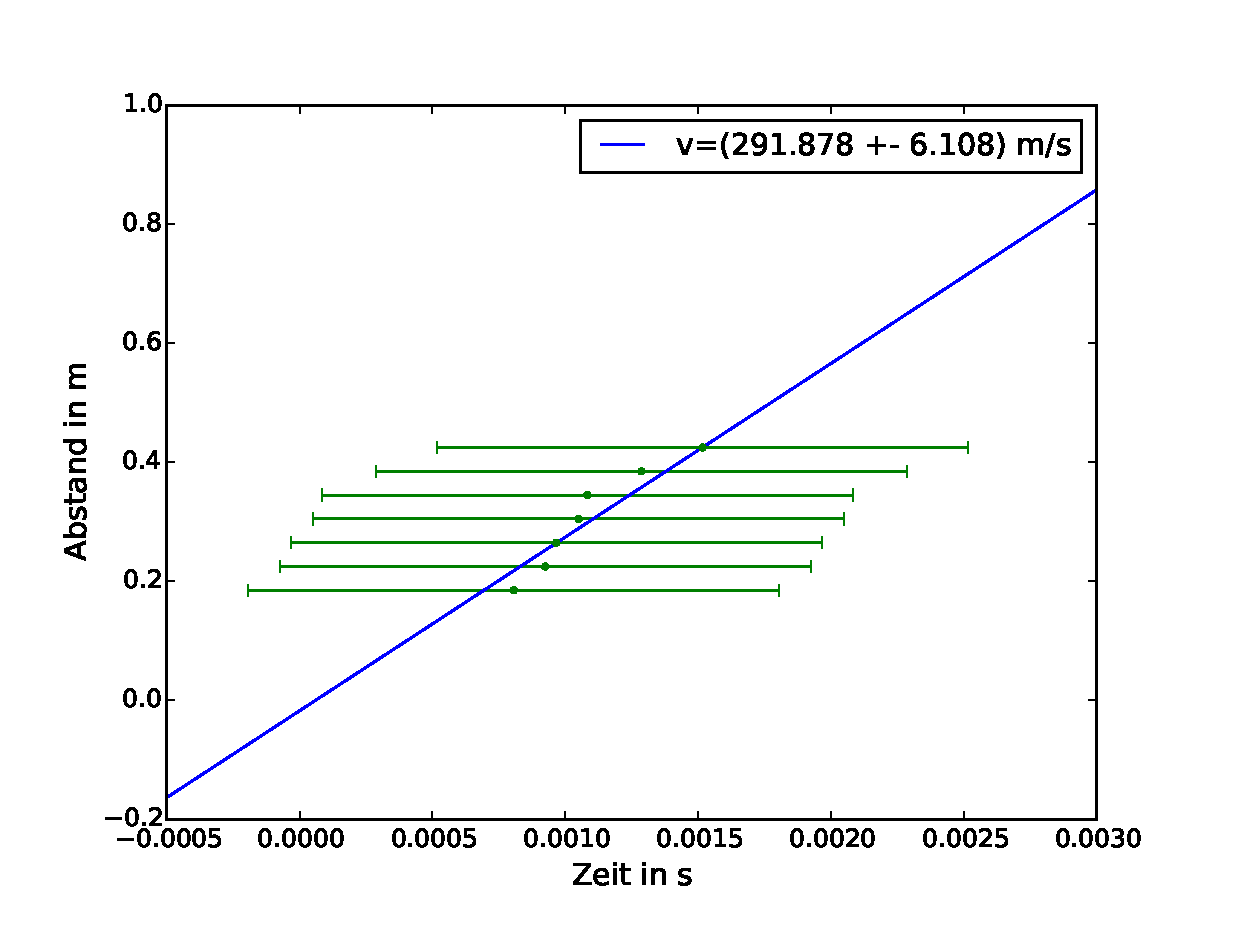
\includegraphics[scale=0.3]{Bilder/Linreg-Laufzeit.eps}
%\caption{Lineare Regression durch die Mittelwerte der Cassy-Messung mit ihren Fehlern}
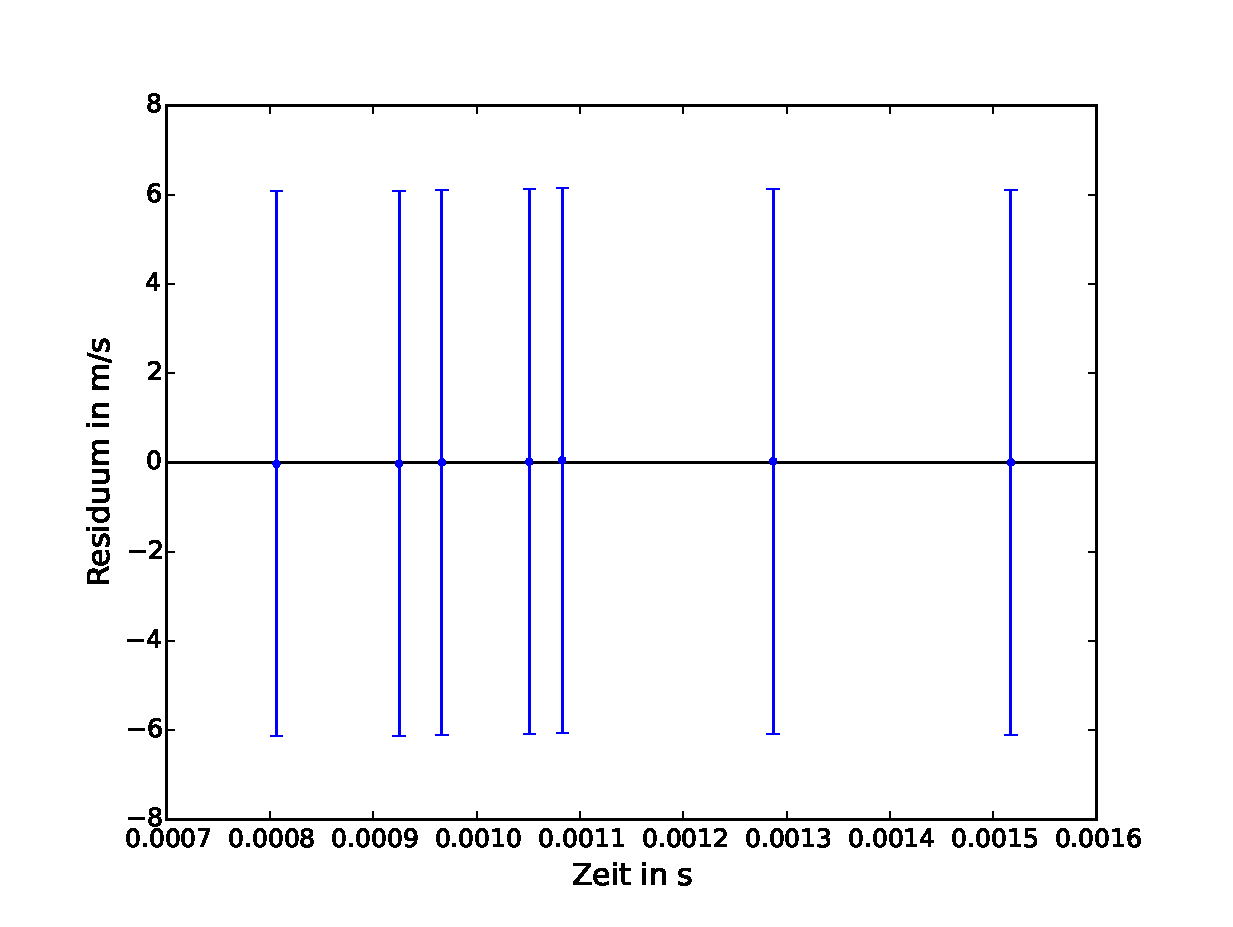
\includegraphics[scale=0.3]{Bilder/Residuen-Laufzeit.eps}
%\caption{Residuen des Fits, der Cassy-Messung}
\end{figure}
\begin{itemize}
\item $\chi^2$ pro Freiheitsgrad $=5.677$
\end{itemize}
\end{frame}
\begin{frame}
\begin{figure}[H]
\centering
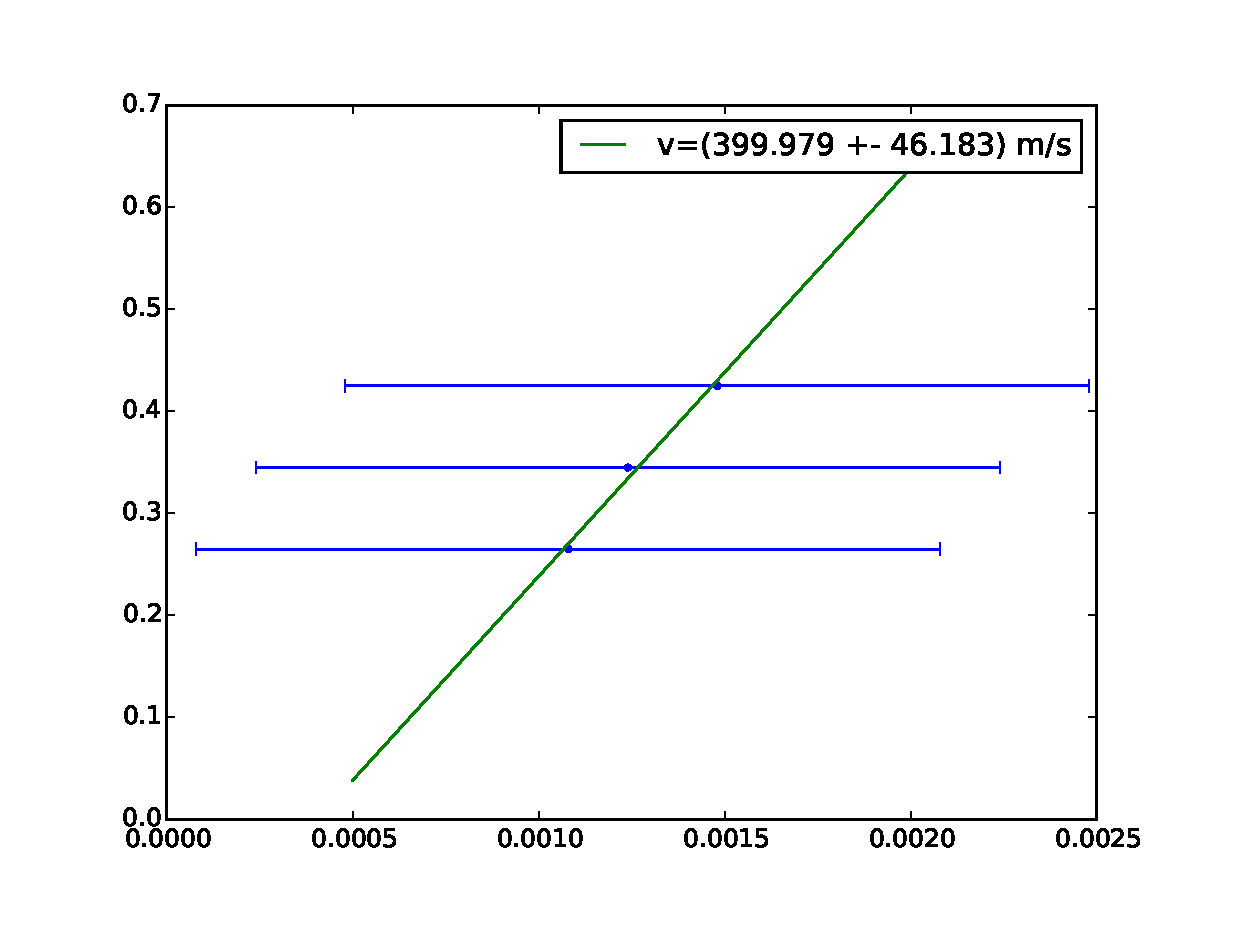
\includegraphics[scale=0.3]{Bilder/Linreg-Oszi.eps}
%\caption{$\chi^2$ pro Freiheitsgrad $=0.664$}
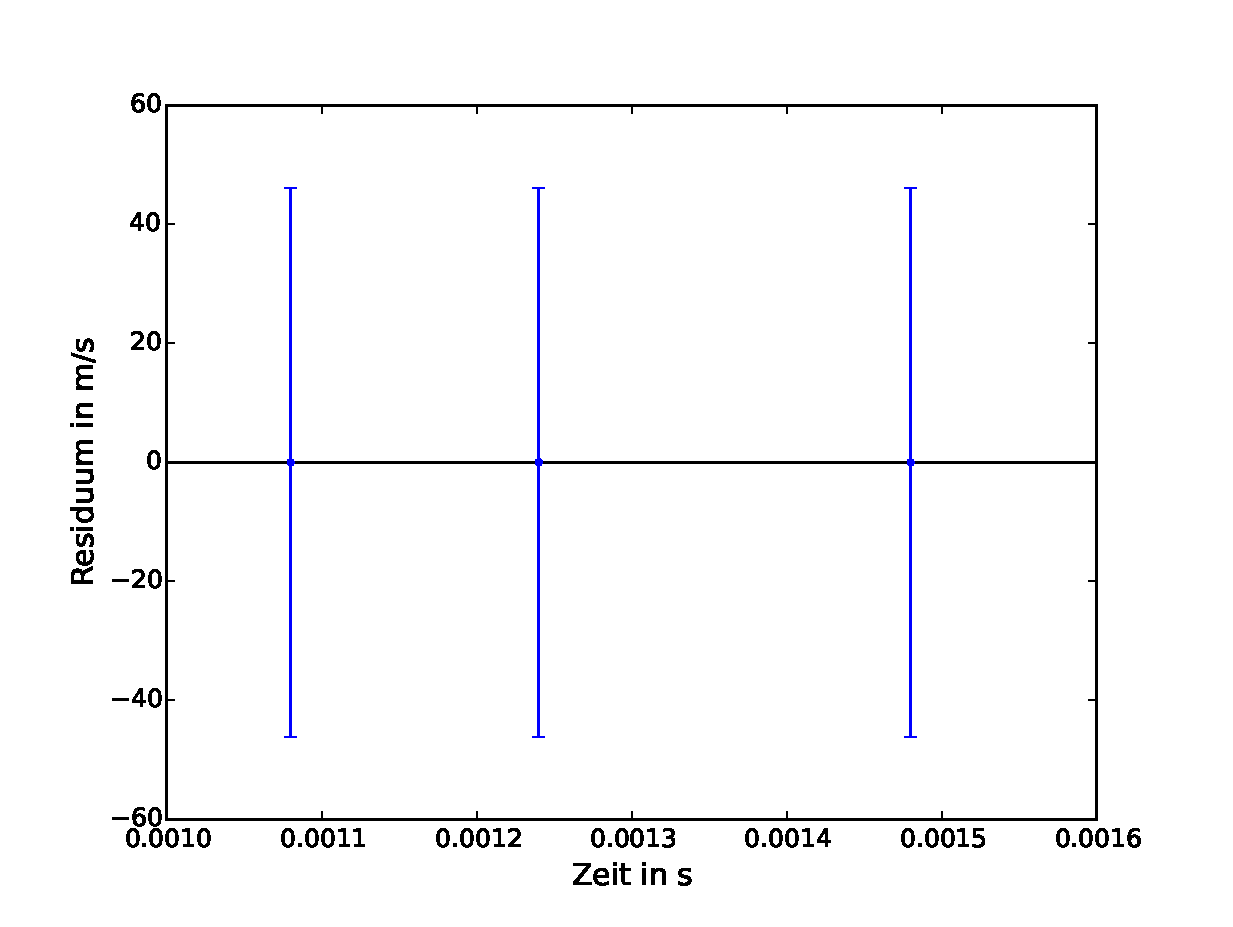
\includegraphics[scale=0.3]{Bilder/Residuen-Oszi.eps}
%\caption{Residuen des Fits der Oszilloskop-Messung}
\end{figure}
\begin{itemize}
\item $\chi^2$ pro Freiheitsgrad $=0.664$
\end{itemize}
\end{frame}
\subsection{Fazit}
\begin{frame}
\begin{itemize}
\item Literaturwert: $344.98 \, \frac{m}{s}$
\item Cassy: $v=(291.878 \pm 6.108) \frac{m}{s} \rightarrow 8\sigma$ Abweichung
\item Oszilloskop: $v=(399.979 \pm 46.183)\frac{m}{s}\rightarrow 1\sigma$ Abweichung
\end{itemize}
\end{frame}

%\begin{frame}
%\tableofcontents
%\end{frame}


\section{Variation der Frequenz}
\subsection{Versuchsbeschreibung}
\begin{frame}{Variation der Frequenz}
\begin{equation*}
f_n = \frac{n\cdot v}{2\cdot L}
\end{equation*}
\begin{itemize}
\item grob Resonanzfrequenzen vermessen
\item danach deutlich mehr Messpunkte
\end{itemize} 
\end{frame}

\subsection{Aufbau und Durchführung}
\begin{frame}
\begin{figure}[H]
\centering
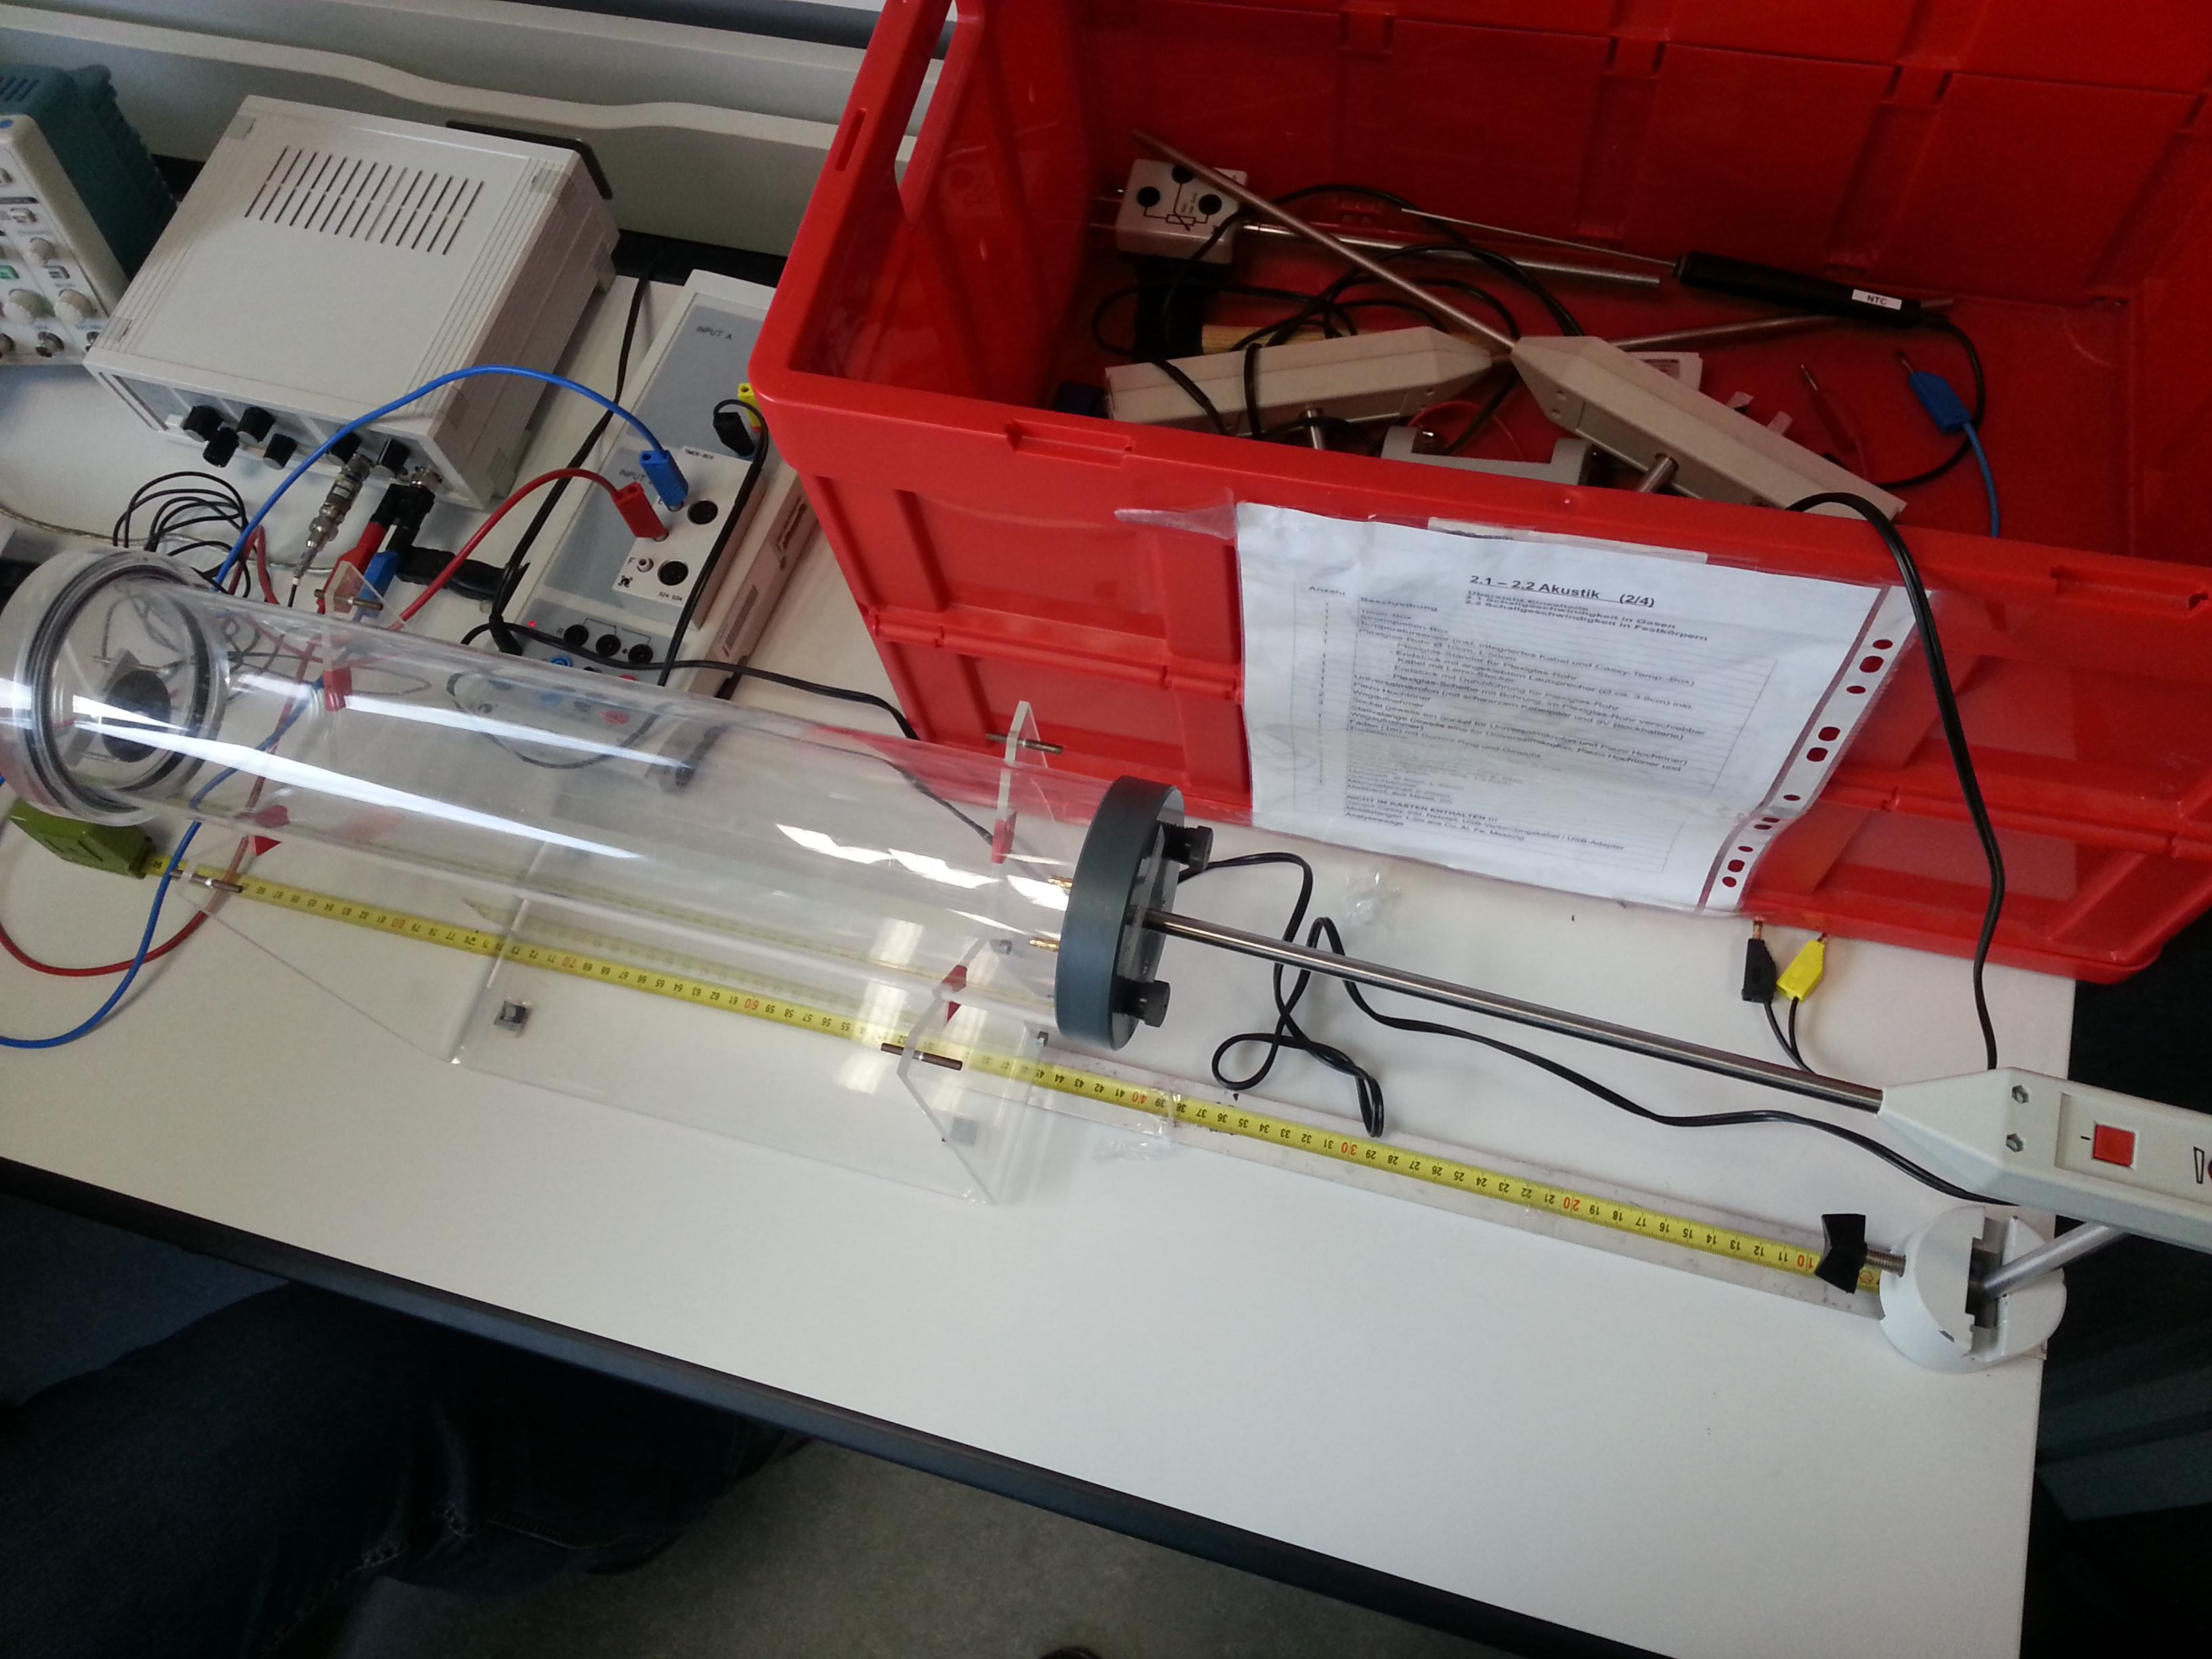
\includegraphics[scale=0.08]{Bilder/Frequenzvariation3.jpg}
\end{figure}
\end{frame}

\subsection{Auswertung}
\begin{frame}
\begin{figure}[H]
\centering
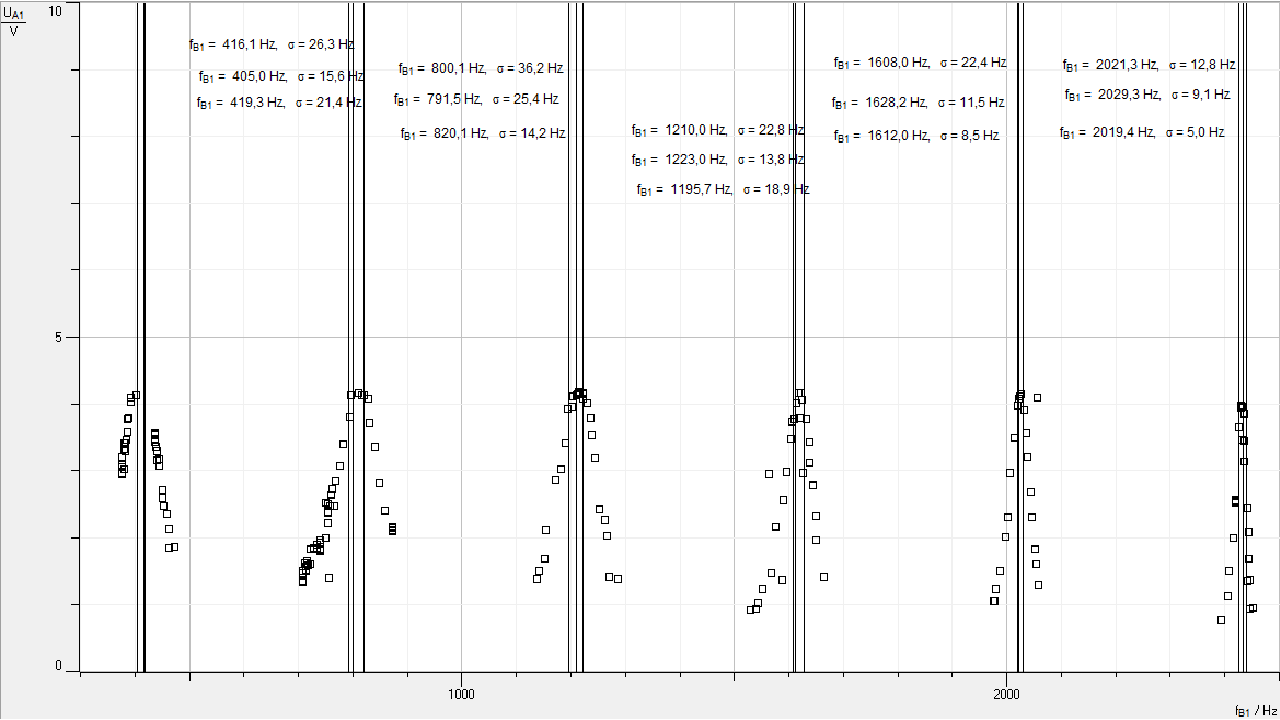
\includegraphics[scale=0.3]{Bilder/vermessung_variation_genau.png}
\end{figure}
\end{frame}

\begin{frame}
\begin{itemize}
\item $L=42.5 cm \hspace{1cm} \sigma_{L} = 1 mm$
\end{itemize}
\begin{table}[H]
\begin{tabular}{c|c|c|c|c|c|c}
$f_{res}$ &400&800&1200&1600&2000&2400\\ 
\hline 
$f_{mean}$ & 412.92 & 812.80 & 1206.97 & 1614.70 & 2030.07 & 2437.33 \\ 
\hline 
$\sigma_{f_{mean}}$ & 6.94 & 16.00 & 11.16 & 18.21 & 10.90 & 14.32 \\ 
\end{tabular}
\caption{Mittelwerte und deren Fehler (alle Angaben in Hz)} 
\end{table}

\end{frame}

\begin{frame}
\begin{figure}[H]
\centering
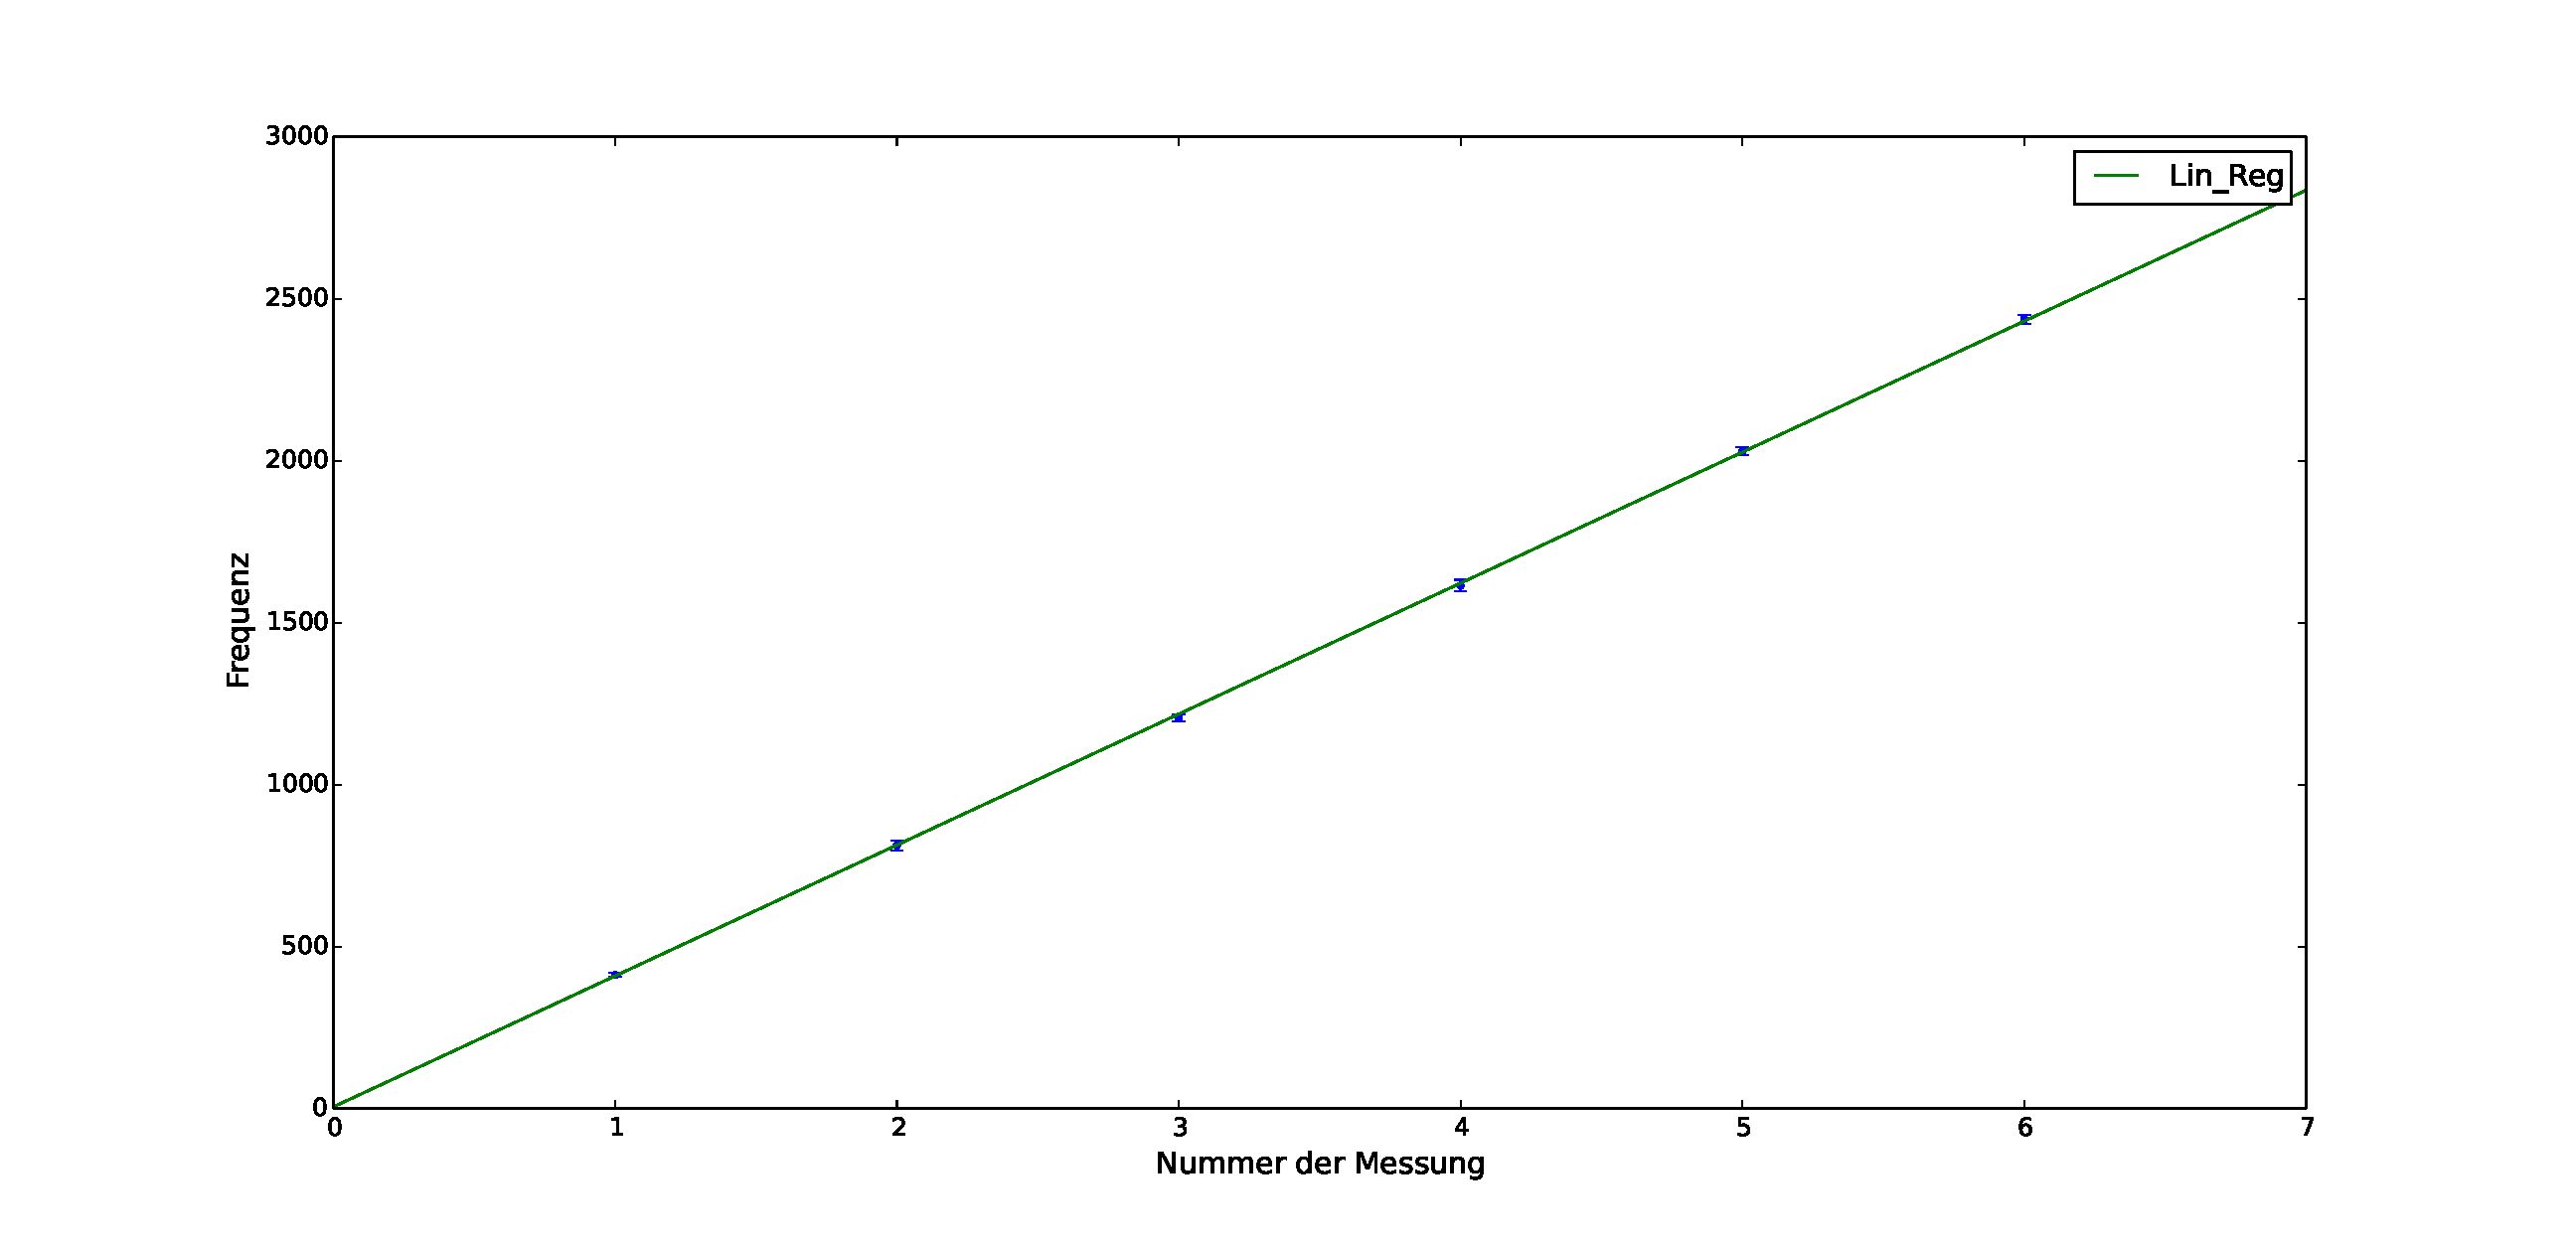
\includegraphics[scale=0.25]{Bilder/Lin_reg_variation_neu.eps}
\end{figure}

\begin{itemize}
\item $a=404.26 \frac{1}{s}, \hspace{1cm} \sigma_a = 2.45 \frac{1}{s}, \hspace{1cm} \frac{\chi^2}{f} = 0.43$
\end{itemize}
\end{frame}

\begin{frame}
\begin{figure}[H]
\centering
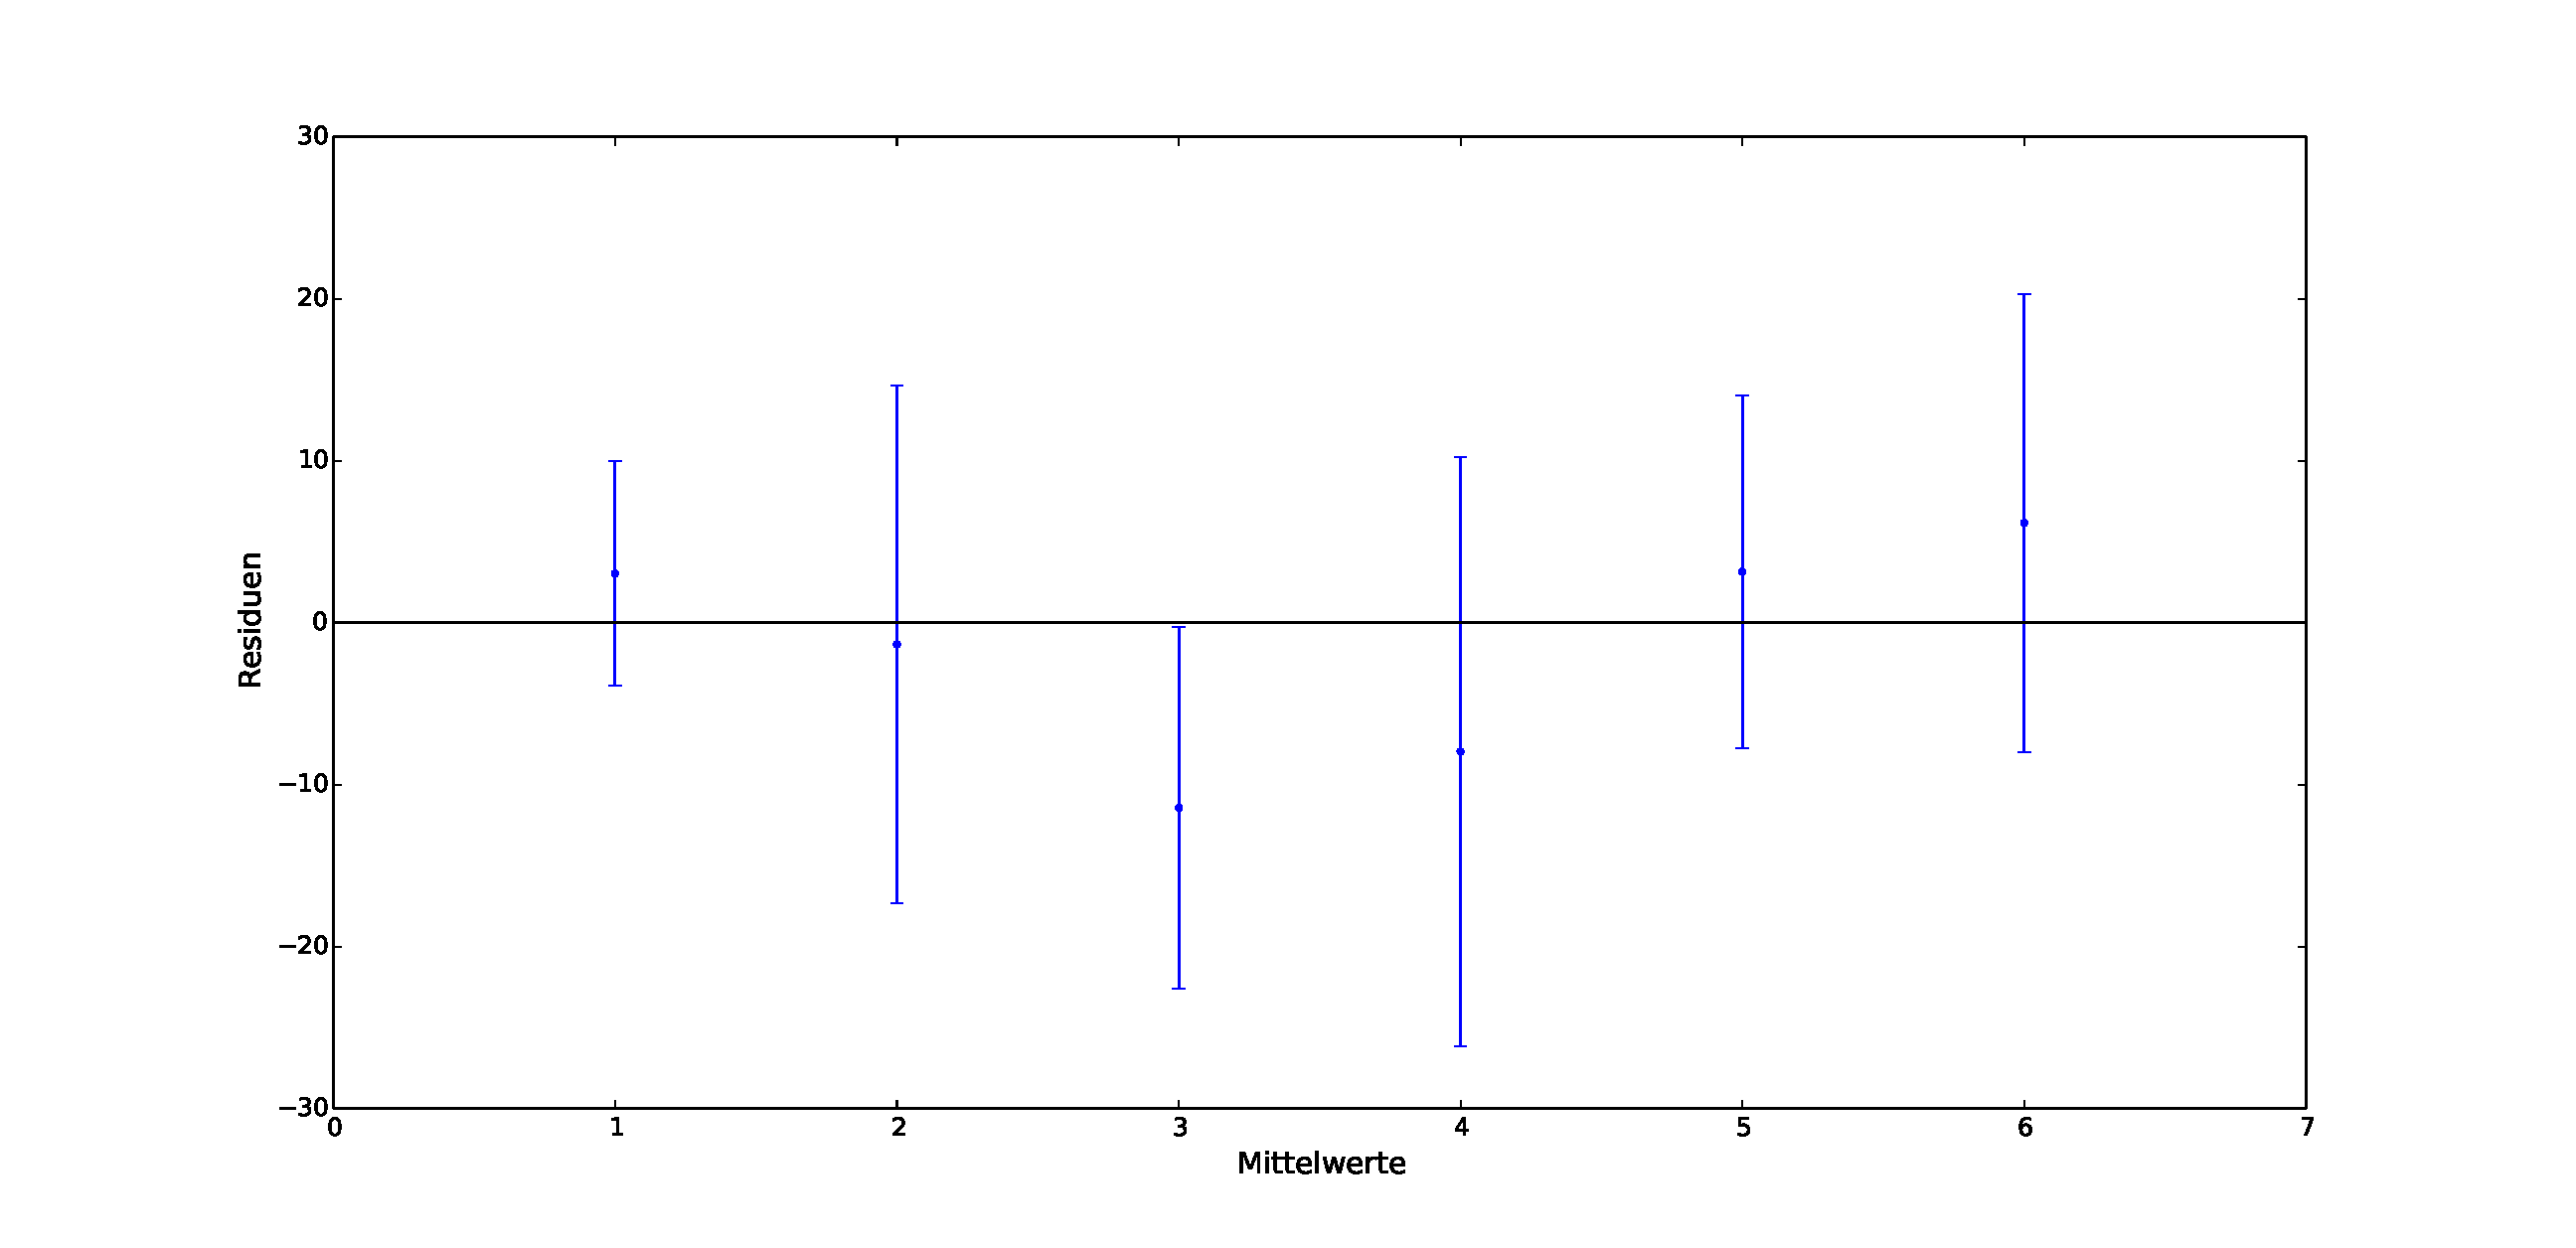
\includegraphics[scale=0.25]{Bilder/Residuen_Variation_Frequenzen.eps}
\end{figure}
\end{frame}


\subsection{Fazit}
\begin{frame}
\begin{equation*}
v=a\cdot 2L
\end{equation*}
\begin{equation*}
\sigma_v = v\cdot \sqrt{(\frac{\sigma_a}{a})^2+(\frac{\sigma_L}{L})^2}
\end{equation*}

\begin{equation*}
v = 343.46 \pm 2.08\,\frac{m}{s}
\end{equation*}.
\begin{itemize}
\item $v_{lit}=344.98\,\frac{m}{s}$
\item $\Rightarrow 1 \sigma$ Abweichung
\\
\item  $\frac{\chi^2}{f} = 0.43$
\end{itemize}
\end{frame}

\section{Vermessung der stehenden Welle}
\subsection{Versuchsbeschreibung}
\begin{frame}{Vermessung der stehenden Welle}
\begin{itemize}
\item $v_{Schall} = \lambda\cdot f$
\item messen des Schalldrucks um charakteristische Punkte der stehenden Welle aufzuzeichnen
\end{itemize}
\end{frame}

\subsection{Aufbau und Durchführung}
\begin{frame}
\begin{figure}[H]
\centering
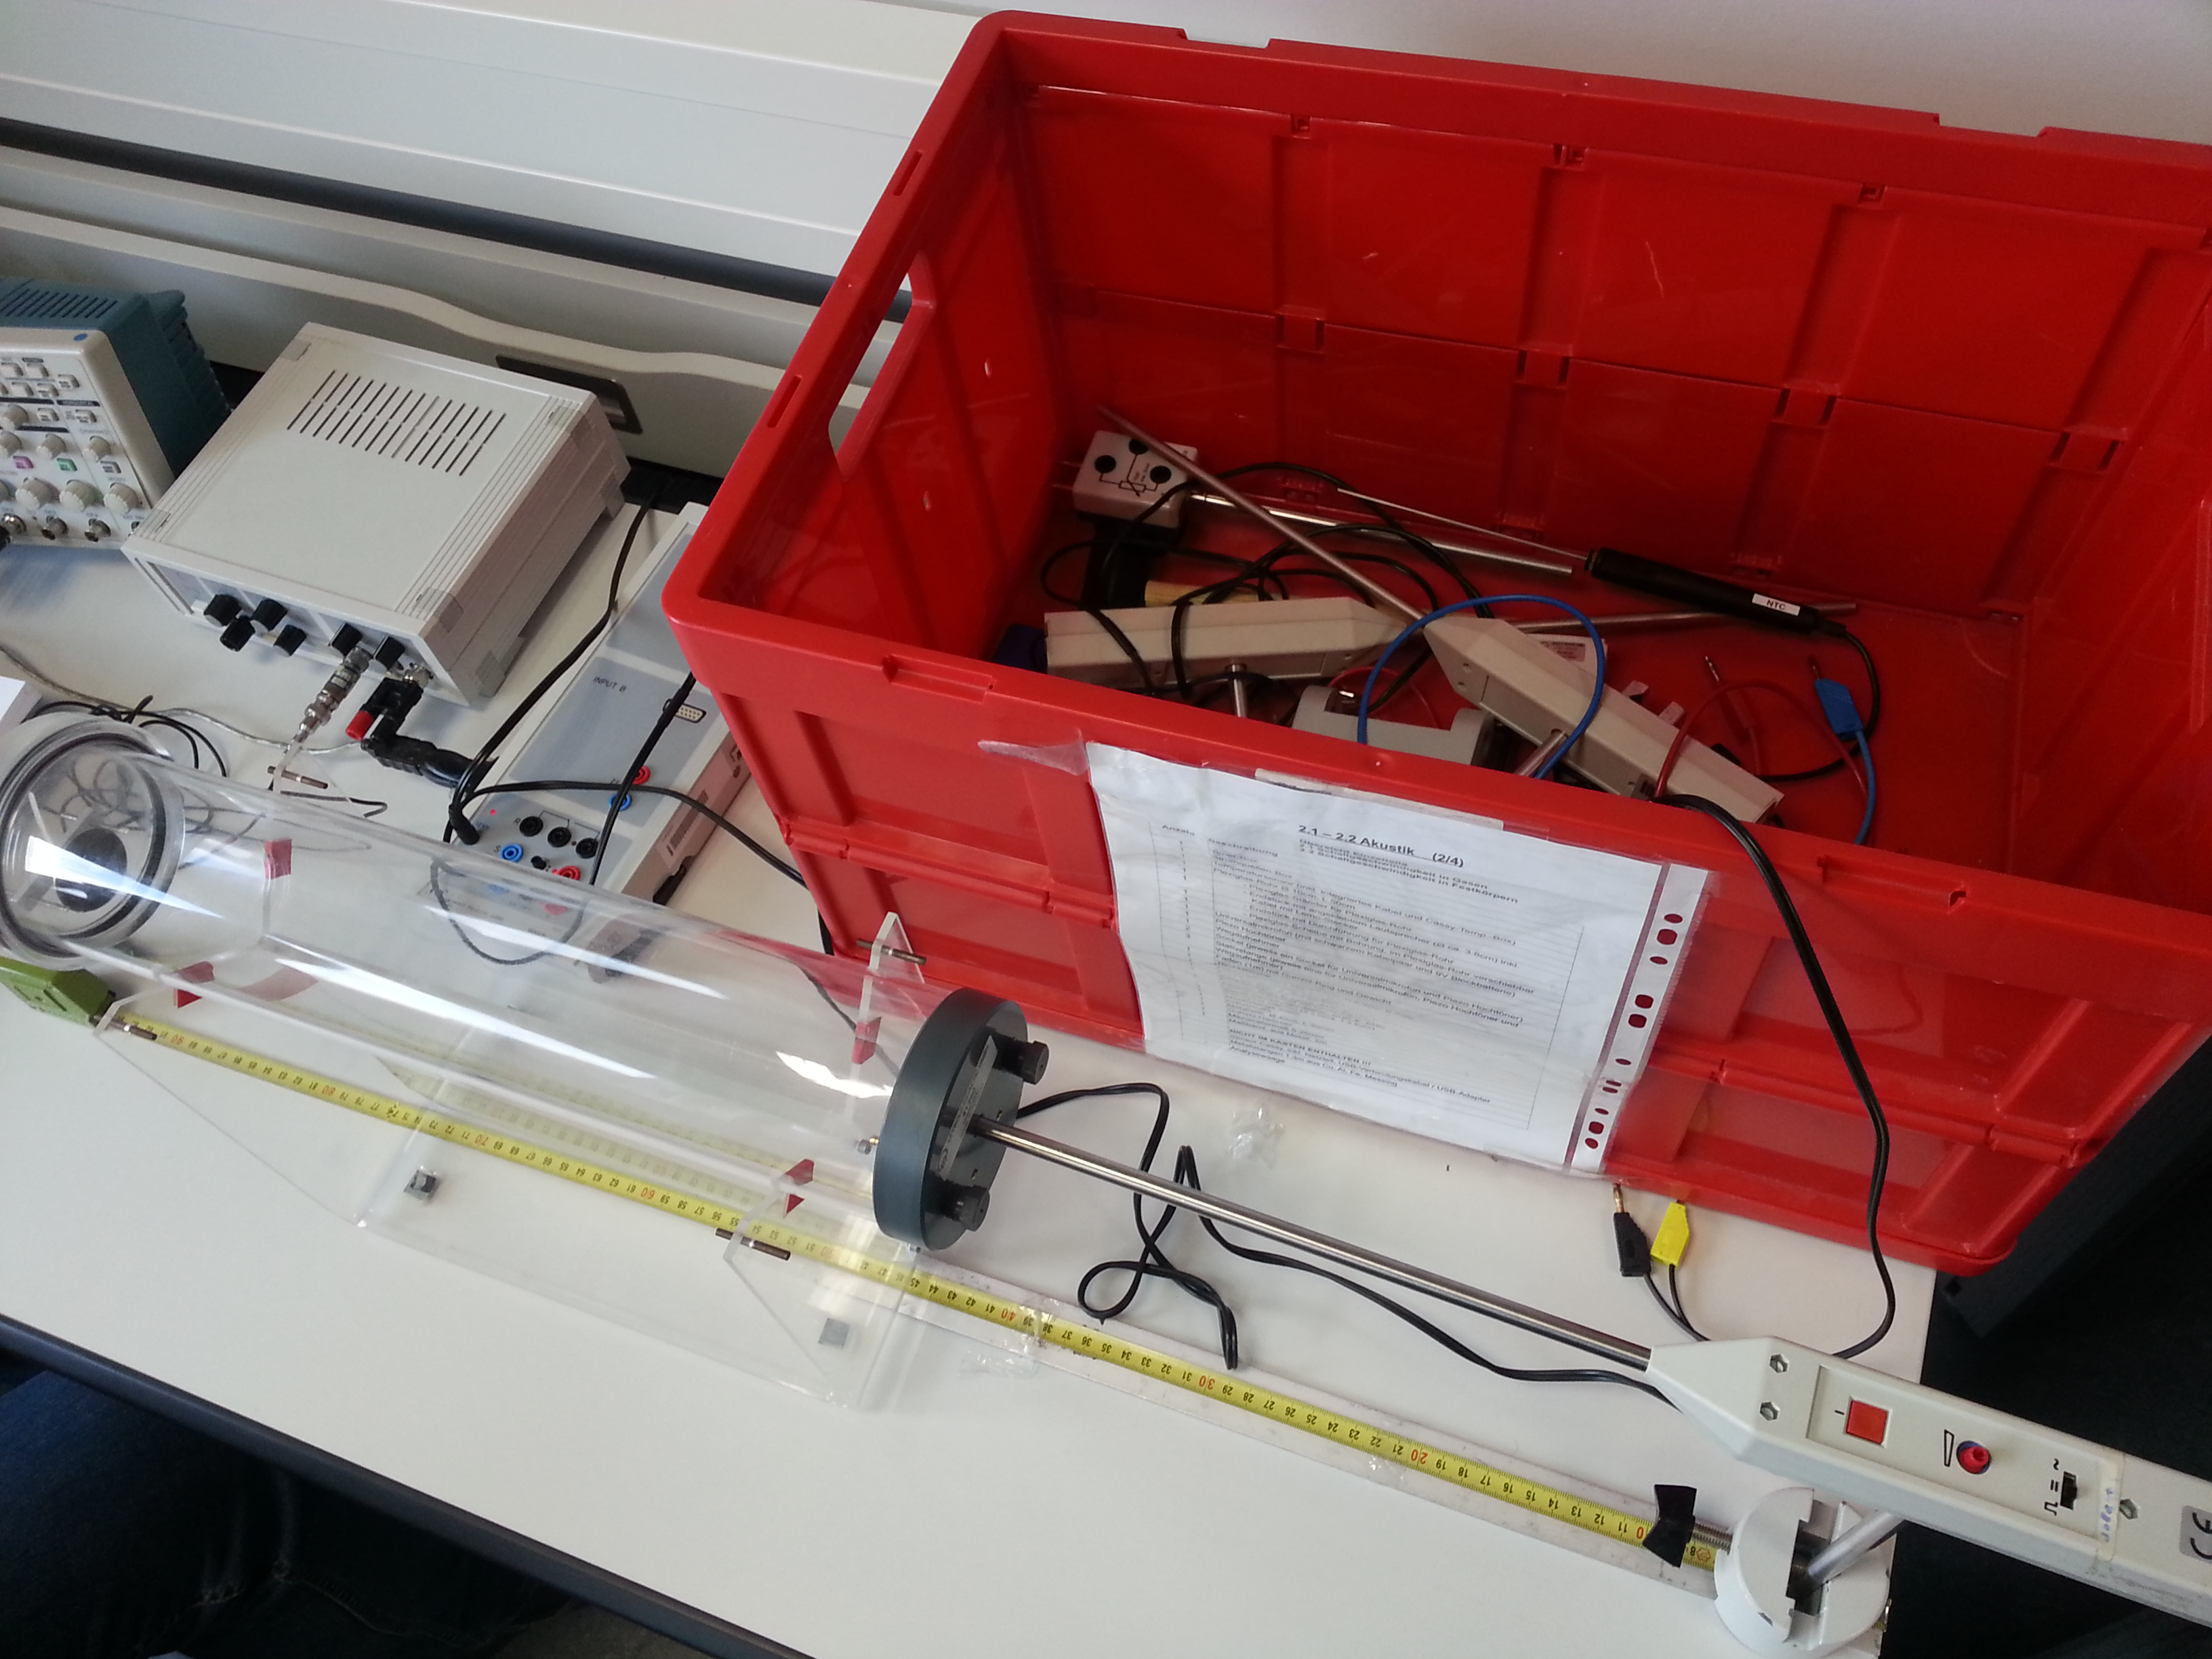
\includegraphics[scale=0.08]{Bilder/Druckknoten-Messung3.jpg}
\end{figure}
\end{frame}

\begin{frame}
\begin{figure}[H]
\centering
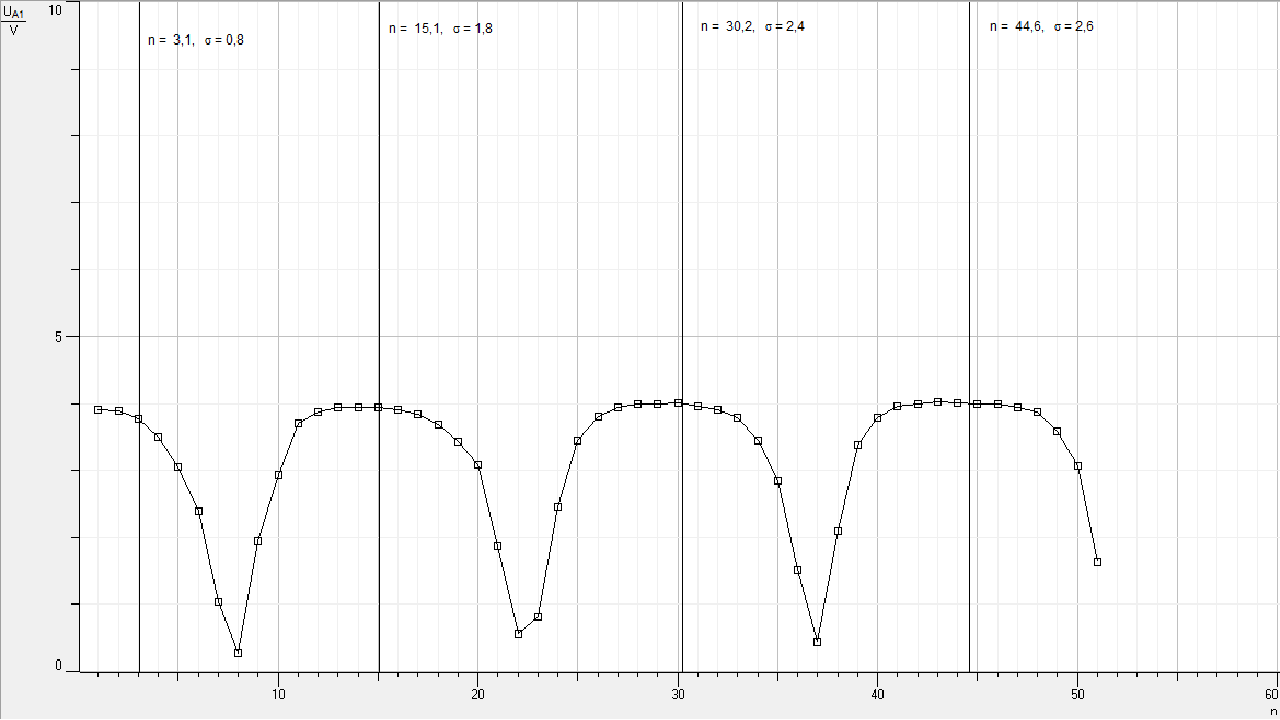
\includegraphics[scale=0.25]{Bilder/baeuche.png}
\caption{$L = (0.025 + n\cdot 0.005) - 0.425$ in m}
\end{figure}
\end{frame}

\subsection{Auswertung}
\begin{frame}
\begin{table}[H]
\begin{tabular}{c|c|c}
Position Bauch N & Messpunkt n & Länge [m] \\ 
\hline 
1.5 & 1 & 0.395 \\ 
2.5 & 15 & 0.325 \\ 
3.5 & 30 & 0.25 \\ 
4.5 & 45 & 0.175 \\ 
\end{tabular}
\caption{Druckbäuche für $f = 2400\,$Hz, mit $\sigma_l = 0.0028\,$m}
\end{table}
\end{frame}

\begin{frame}
\begin{figure}[H]
\centering
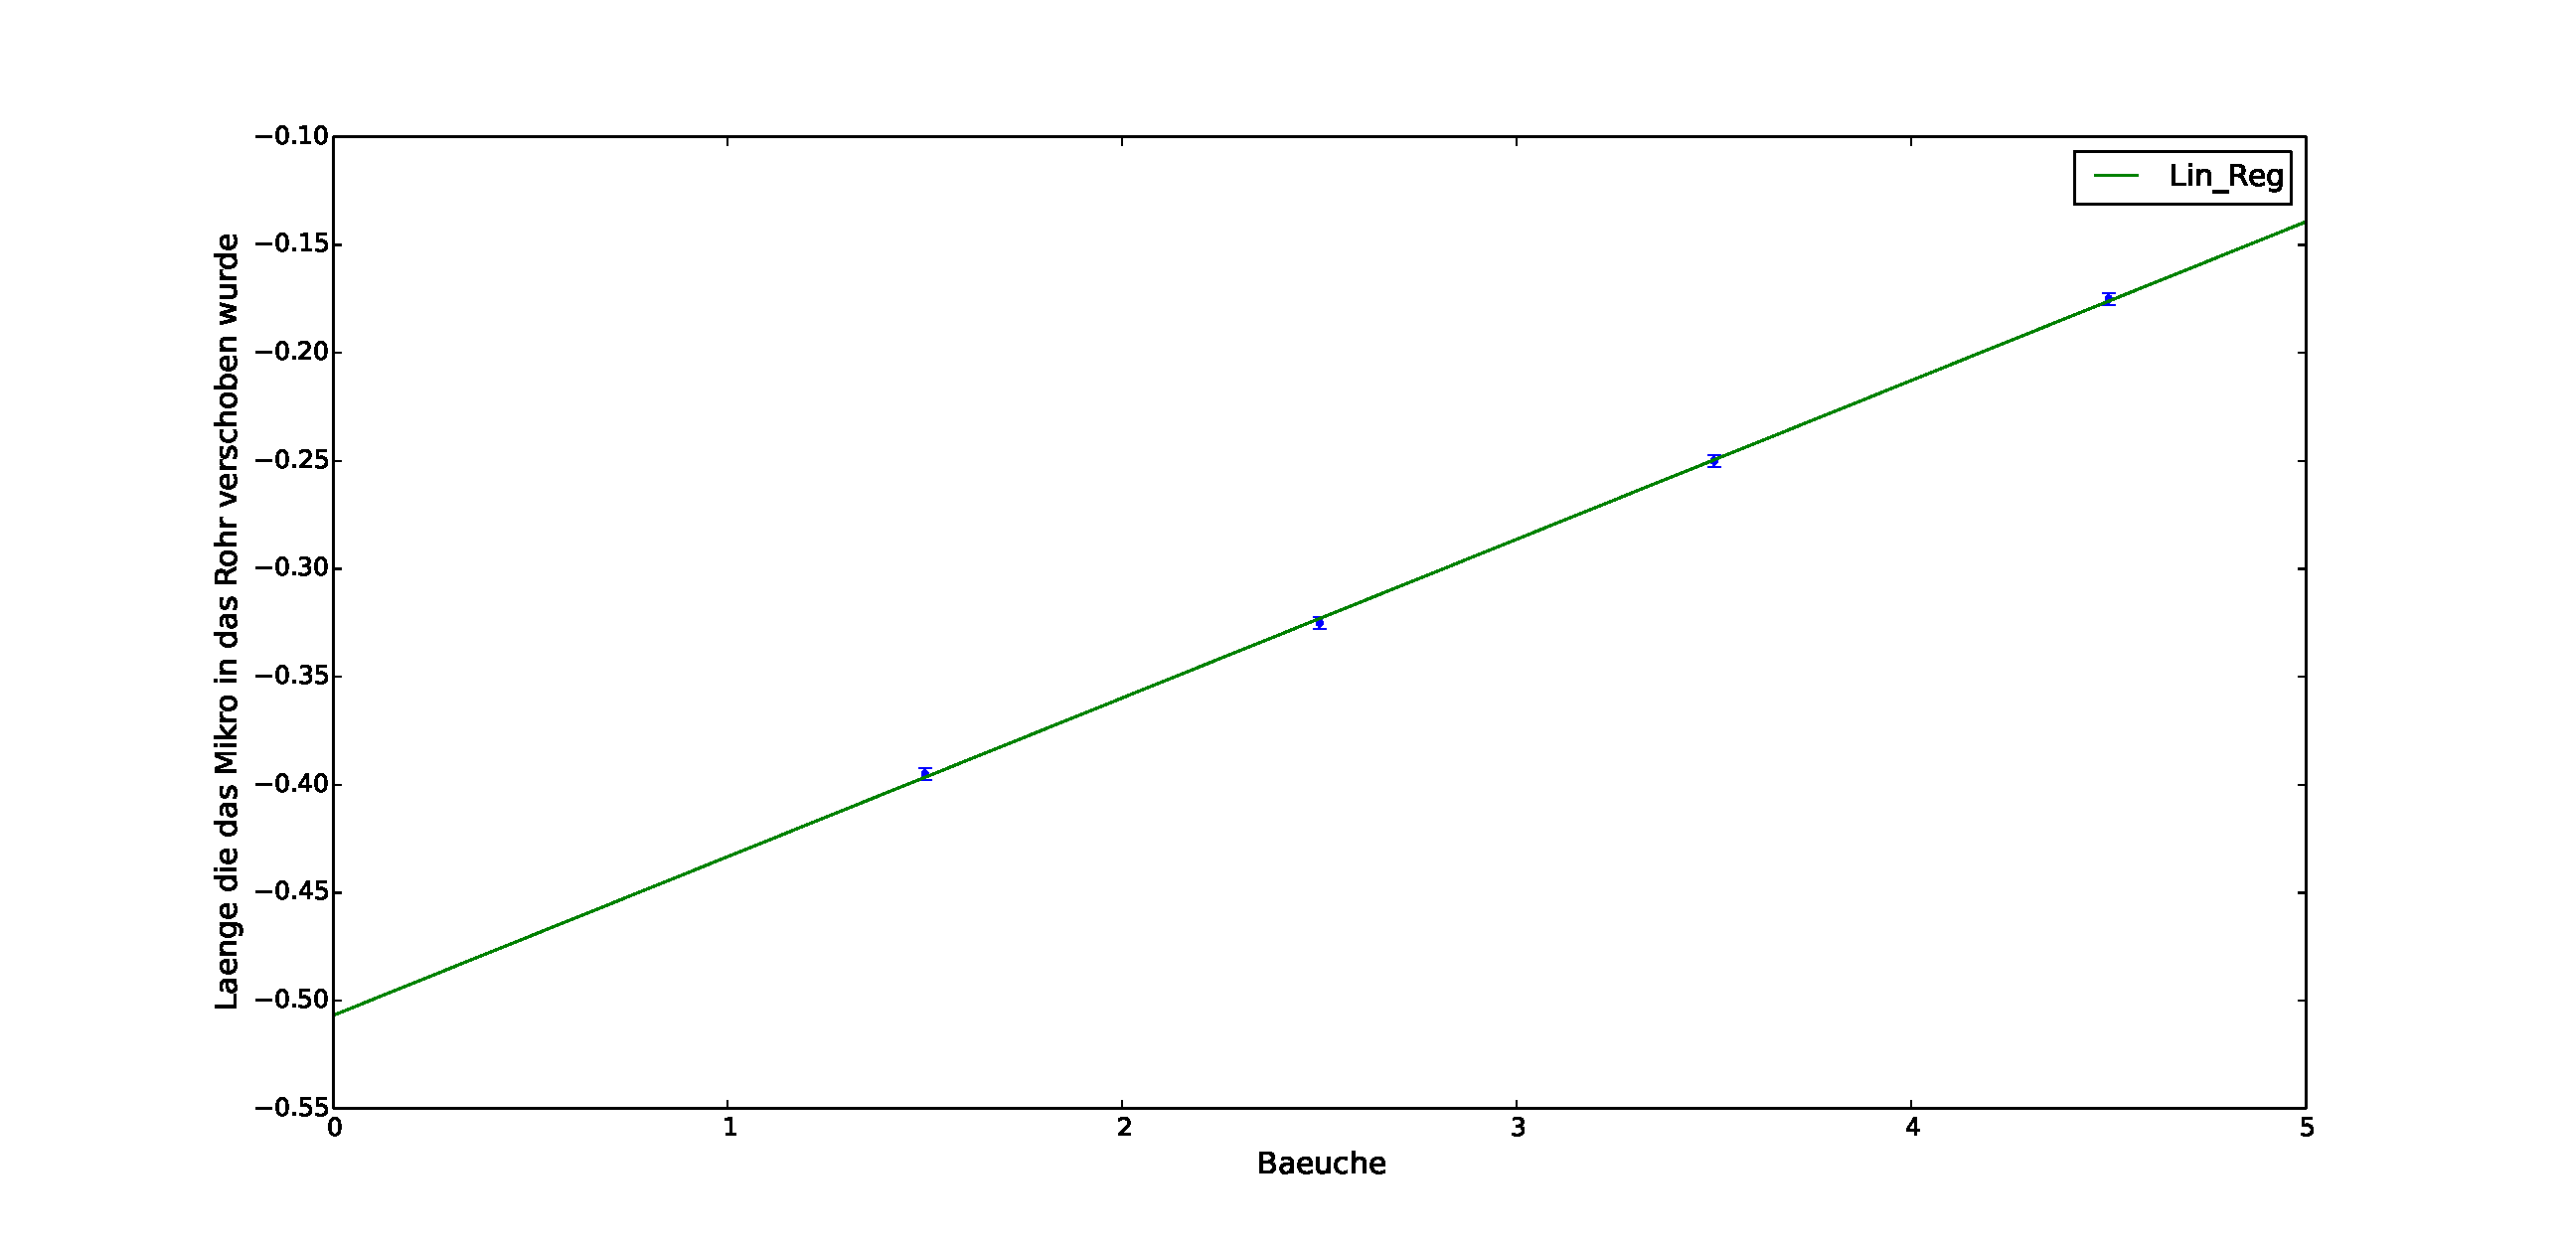
\includegraphics[scale=0.25]{Bilder/linreg_stehende_welle.eps}
\end{figure}
\begin{itemize}
\item $\frac{\chi^2}{f} = 0.47, \hspace{1cm} a=0.0735$
\end{itemize}
\end{frame}

\begin{frame}
\begin{figure}[H]
\centering
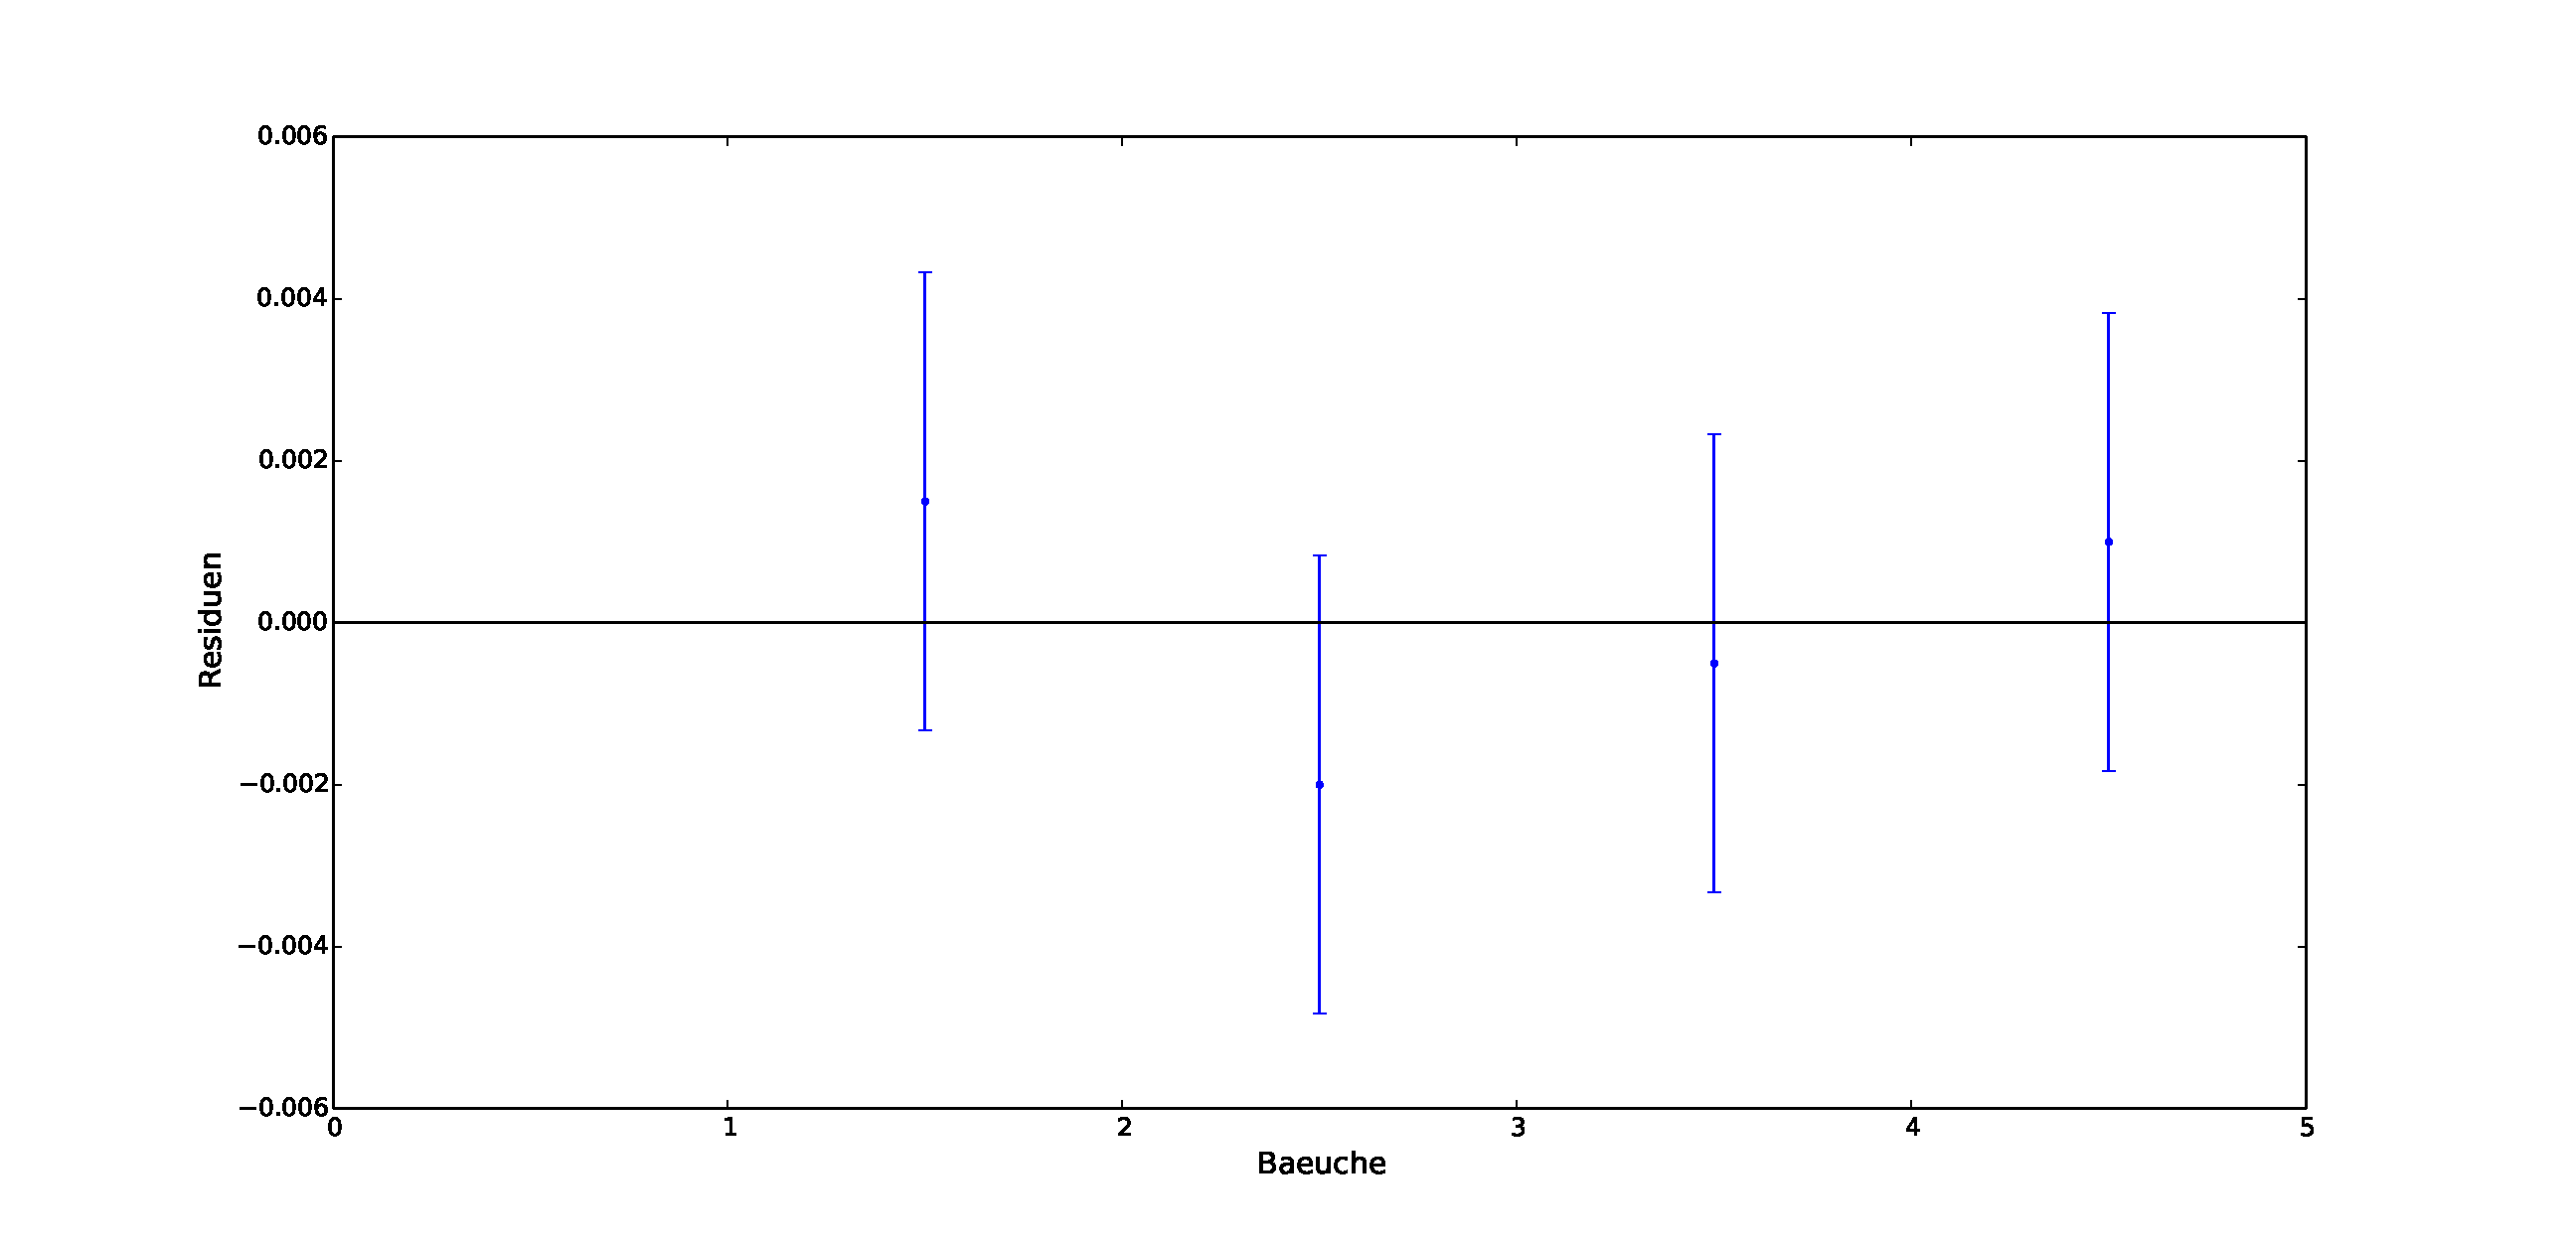
\includegraphics[scale=0.25]{Bilder/residuen_stehende_welle.eps}
\end{figure}
\end{frame}

\begin{frame}{Fehlerrechnung und Ergebnis}
\begin{equation*}
v=\lambda f
\end{equation*}
\begin{equation*}
\sigma_{v} = \sqrt{f^2\cdot\sigma_{\lambda}^2 + \lambda^2\cdot\sigma_{f}^2}
\end{equation*}
mit $\sigma_{\lambda} = 0.0025\,$m 
\begin{itemize}
\item $v = 352.8 \pm 4.5\,\frac{m}{s}$
\end{itemize}
\end{frame}

\subsection{Fazit}
\begin{frame}{Fazit}
\begin{itemize}
\item unser Wert: $v = 352.8 \pm 4.5\,\frac{m}{s}$ 
\item Literaturwert: $v = 344.98\,\frac{m}{s}$
\item innerhalb von $2 \sigma$
\item Güte unserer Anpassung: $\frac{\chi^2}{f} = 0.47$
\end{itemize}
\end{frame}

\section{Fazit}
\begin{frame}{Fazit}
\begin{tabular}{|c|c|c|}
\hline 
Methode & v in m/s & $\sigma_v$ in m/s \\ 
\hline 
Laufzeit Cassy & 291.8 & 6.1 \\ 
\hline 
Laufzeit Oszilloskop & 400.0 & 46.2 \\ 
\hline 
Variation d. Frequenz & 343.5 & 2.1 \\ 
\hline 
Verm. der stehenden Welle & 352.8 & 4.5 \\ 
\hline 
Literaturwert & 344.98 &  \\ 
\hline 
\end{tabular} 
\end{frame}

%\begin{frame}
%\tableofcontents
%\end{frame}

\section{Schallgeschwindigkeit in Festkörpern}
\subsection{Aufbau}
\begin{frame}{Schallgeschwindigkeit in Festkörpern}
\begin{figure}[H]
\centering
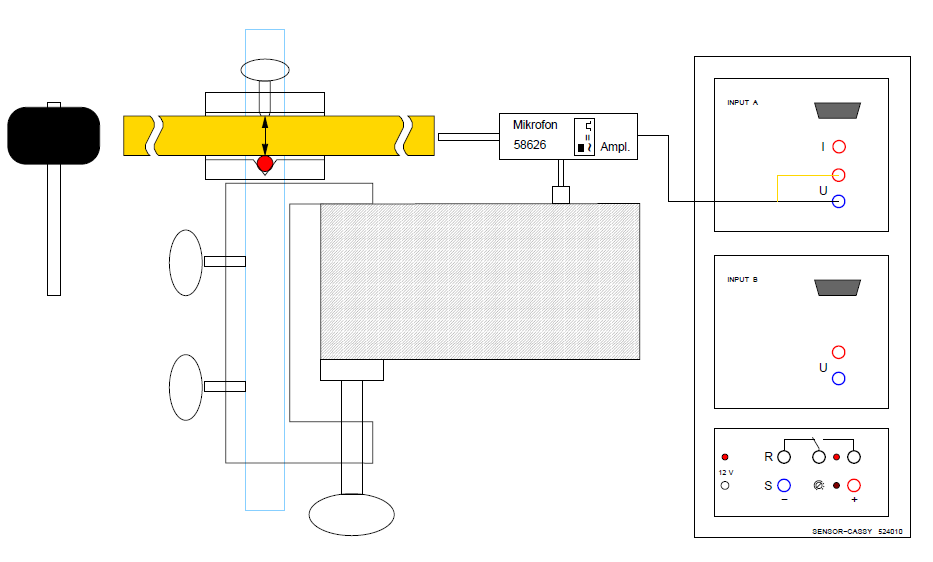
\includegraphics[scale=0.35]{Bilder/Versuchsaufbau_Skript.PNG}
\label{Stange}
\end{figure}
\begin{equation*}
v=\sqrt{\frac{E}{\rho}}, \hspace{1cm} E= \rho\cdot f^2\cdot 4L^2, \hspace{1cm} \rho=\frac{M}{V}=\frac{4\cdot M}{L\cdot \pi D^2}
\end{equation*}
\end{frame}
\subsection{Rohdaten}
\begin{frame}
\begin{figure}[H]
\centering
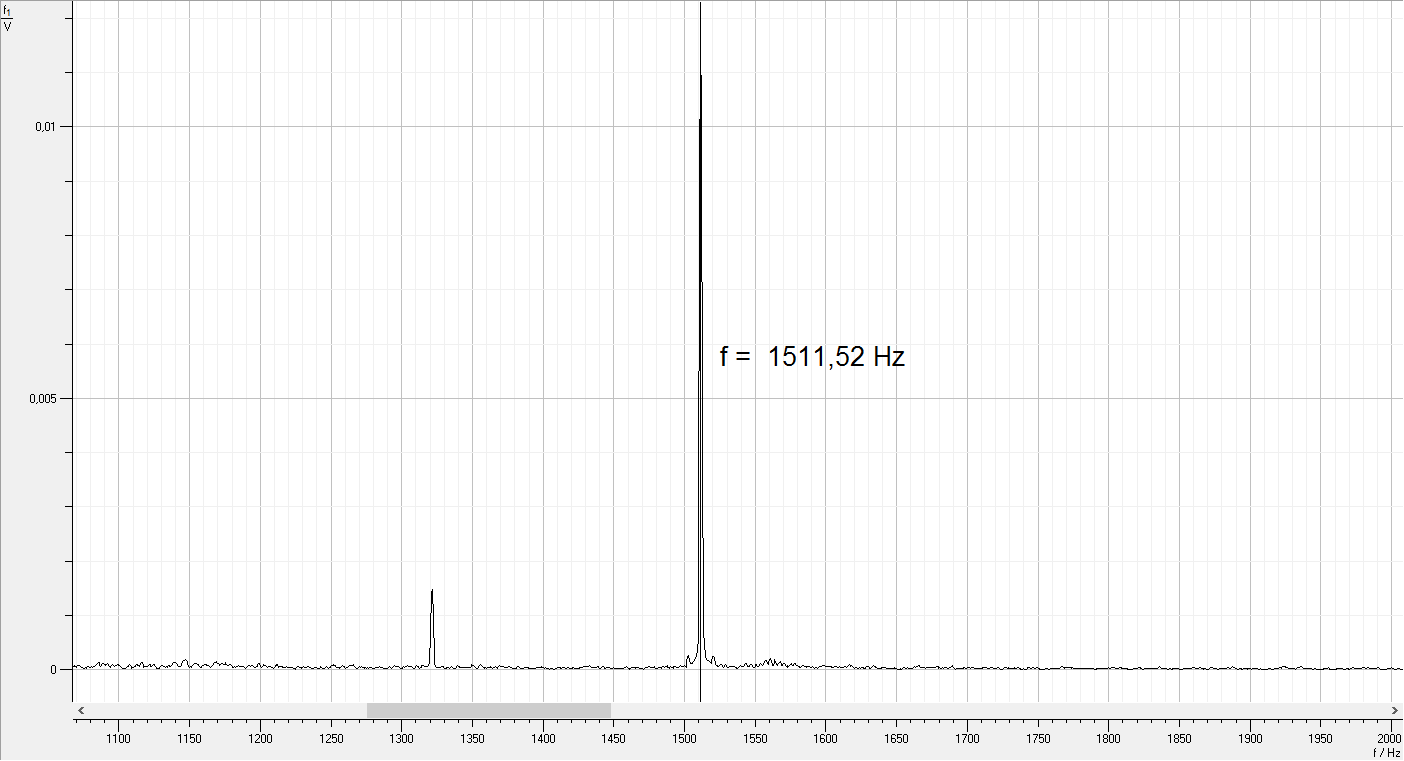
\includegraphics[scale=0.3]{Bilder/Beispiel_Cassy_Cu.png}
\caption{Frequenz aus FFT (Stange 1)}
\end{figure}
\end{frame}

\begin{frame}
\begin{table}[H]\centering
\begin{tabular}{c|cccc}
 & Stange 1 & Stange 2 & Stange 3 & Stange 4 \\ 
 \hline
$f_1$ & 1511.52 & 1728.17 & 1884.03 & 1348.48 \\ 
$f_2$ & 1511.54 & 1728.18 & 1884.04 & 1348.50 \\ 
$f_3$ & 1511.52 & 1728.18 & 1884.07 & 1348.49 \\ 
$f_4$ & 1511.53 & 1728.19 & 1884.06 & 1348.50 \\ 
$f_5$ & 1511.51 & 1728.18 & 1884.09 & 1348.50 \\ 
$f_6$ & 1511.53 & 1728.17 & 1884.11 & 1348.54 \\ 
$f_7$ & 1511.54 & 1728.18 & 1884.13 & 1348.55 \\ 
$f_8$ & 1511.51 & 1728.20 & 1884.14 & 1348.55 \\ 
$f_9$ & 1511.51 & 1728.19 & 1884.13 & 1348.52 \\ 
$f_{10}$ & 1511.48 & 1728.20 & 1884.14 & 1348.52 \\
\hline 
$f_{mean}$ & 1511.52 & 1728.18 &  1884.09 & 1348.52 \\ 
$\sigma_{f_{mean}}$ & 0.006 & 0.003 & 0.013 & 0.008 \\ 
\end{tabular}
\end{table}
\end{frame}

\begin{frame}
\begin{table}[H]\centering
\begin{tabular}{c|cccc}
& Stange 1 & Stange 2 & Stange 3 & Stange 4 \\ 
\hline
m in kg & 1.3019 & 1.3249 & 1.1570 & 1.2364 \\ 
L in m & 1.299  & 1.50 & 1.301 & 1.299 \\ 
\end{tabular} 
\end{table}
\begin{align*}
\sigma_m&=0.0001\,kg\\
\sigma_l&=0.5\cdot10^{-2}\,m
\end{align*}
\begin{table}[H]\centering
\begin{tabular}{c|cccc}
 & Stange 1 & Stange 2 & Stange 3 & Stange 4 \\ 
 \hline
$d_{mean}$ & $12.47$ & 12.00 & 11.96 & 1198 \\ 
$\sigma_{d_{mean}}$ & $0.00$ & $4.47\cdot 10^{-3}$ & $4.00\cdot 10^{-3}$ & $5.83\cdot 10^{-3}$ \\ 
\end{tabular} 
\end{table}
\end{frame}

\subsection{Dichte}
\begin{frame}
\begin{equation*}
\rho=\frac{M}{V}=\frac{4\cdot M}{L\cdot \pi D^2}
\end{equation*}
\begin{equation*}
\sigma_{\rho}=\sqrt{(\frac{\sigma_m}{m})^2+(\frac{\sigma_L}{L})^2+(2\cdot \frac{\sigma_d}{d})^2}\cdot \rho
\end{equation*}
\begin{table}[H]\centering
\begin{tabular}{c|cccc}
  & Stange 1 & Stange 2 & Stange 3 & Stange 4 \\ 
  \hline
$\rho$ in $\frac{kg}{m^3}$ & 8206.3 & 7809.3 & 7910.7 & 8446.8 \\ 
$\sigma_{\rho}$ in $\frac{kg}{m^3}$ & 31.6 & 26.7 & 30.9 & 33.9 \\ 
Material & Kupfer & Eisen & Eisen & Messing \\ 
$\rho_{lit}$ in $\frac{kg}{m^3}$ & 8920 & 7874 & 7874 & 8410 \\ 
\end{tabular} 
\end{table}
\end{frame}

\subsection{Elastizitätsmodul}
\begin{frame}
\begin{equation*}
E=4\rho\cdot f^2\cdot  L^2
\end{equation*}
\begin{equation*}
\sigma_{E}=\sqrt{(\frac{\sigma_{\rho}}{\rho})^2+(2\cdot \frac{\sigma_L}{L})^2+(2\cdot \frac{\sigma_f}{f})^2}\cdot E
\end{equation*}

\begin{table}[H]\centering
\begin{tabular}{c|cccc}
 & Stange 1 & Stange 2 & Stange 3 & Stange 4 \\
\hline 
E in GPa & 126.5 & 209.9 & 190.1 & 103.7 \\ 
$\sigma_E$ in GPa & 1.1 & 1.6 & 1.6 & 0.8 \\ 
\end{tabular} 
\end{table}
\end{frame}

\subsection{Schallgeschwindigkeit}
\begin{frame}
\begin{align*}
v=\sqrt{\frac{E}{\rho}}=2fL, \hspace{1cm}
\sigma_v=\sqrt{(\frac{\sigma_f}{f})^2+(\frac{\sigma_L}{L})^2}\cdot v
\end{align*}

\begin{table}[H]\centering
\begin{tabular}{c|cccc}
 & Stange 1 & Stange 2 & Stange 3 & Stange 4 \\ 
\hline
v in $\frac{m}{s}$ & 3926.9 & 5184.6 & 4902.4 & 3503.4 \\ 
$\sigma_{v}$ in $\frac{m}{s}$ & 15.1 & 17.3 & 18.8 & 13.5 \\ 
Material & Kupfer & Eisen & Eisen & Messing \\ 
$v_{Literatur}$ in $\frac{m}{s}$ &$\approx 4660$ & $\approx 5170$ & $\approx 5170$ & $\approx 3500$ \\ 
\end{tabular} 
\end{table}
\end{frame}


\section{Stimmen der Gitarre über Schwebung}
\subsection{Versuchsaufbau für alle Experimente mit der Gitarre}
\begin{frame}{Stimmen der Gitarre über Schwebung}
\begin{figure}[H]
\centering
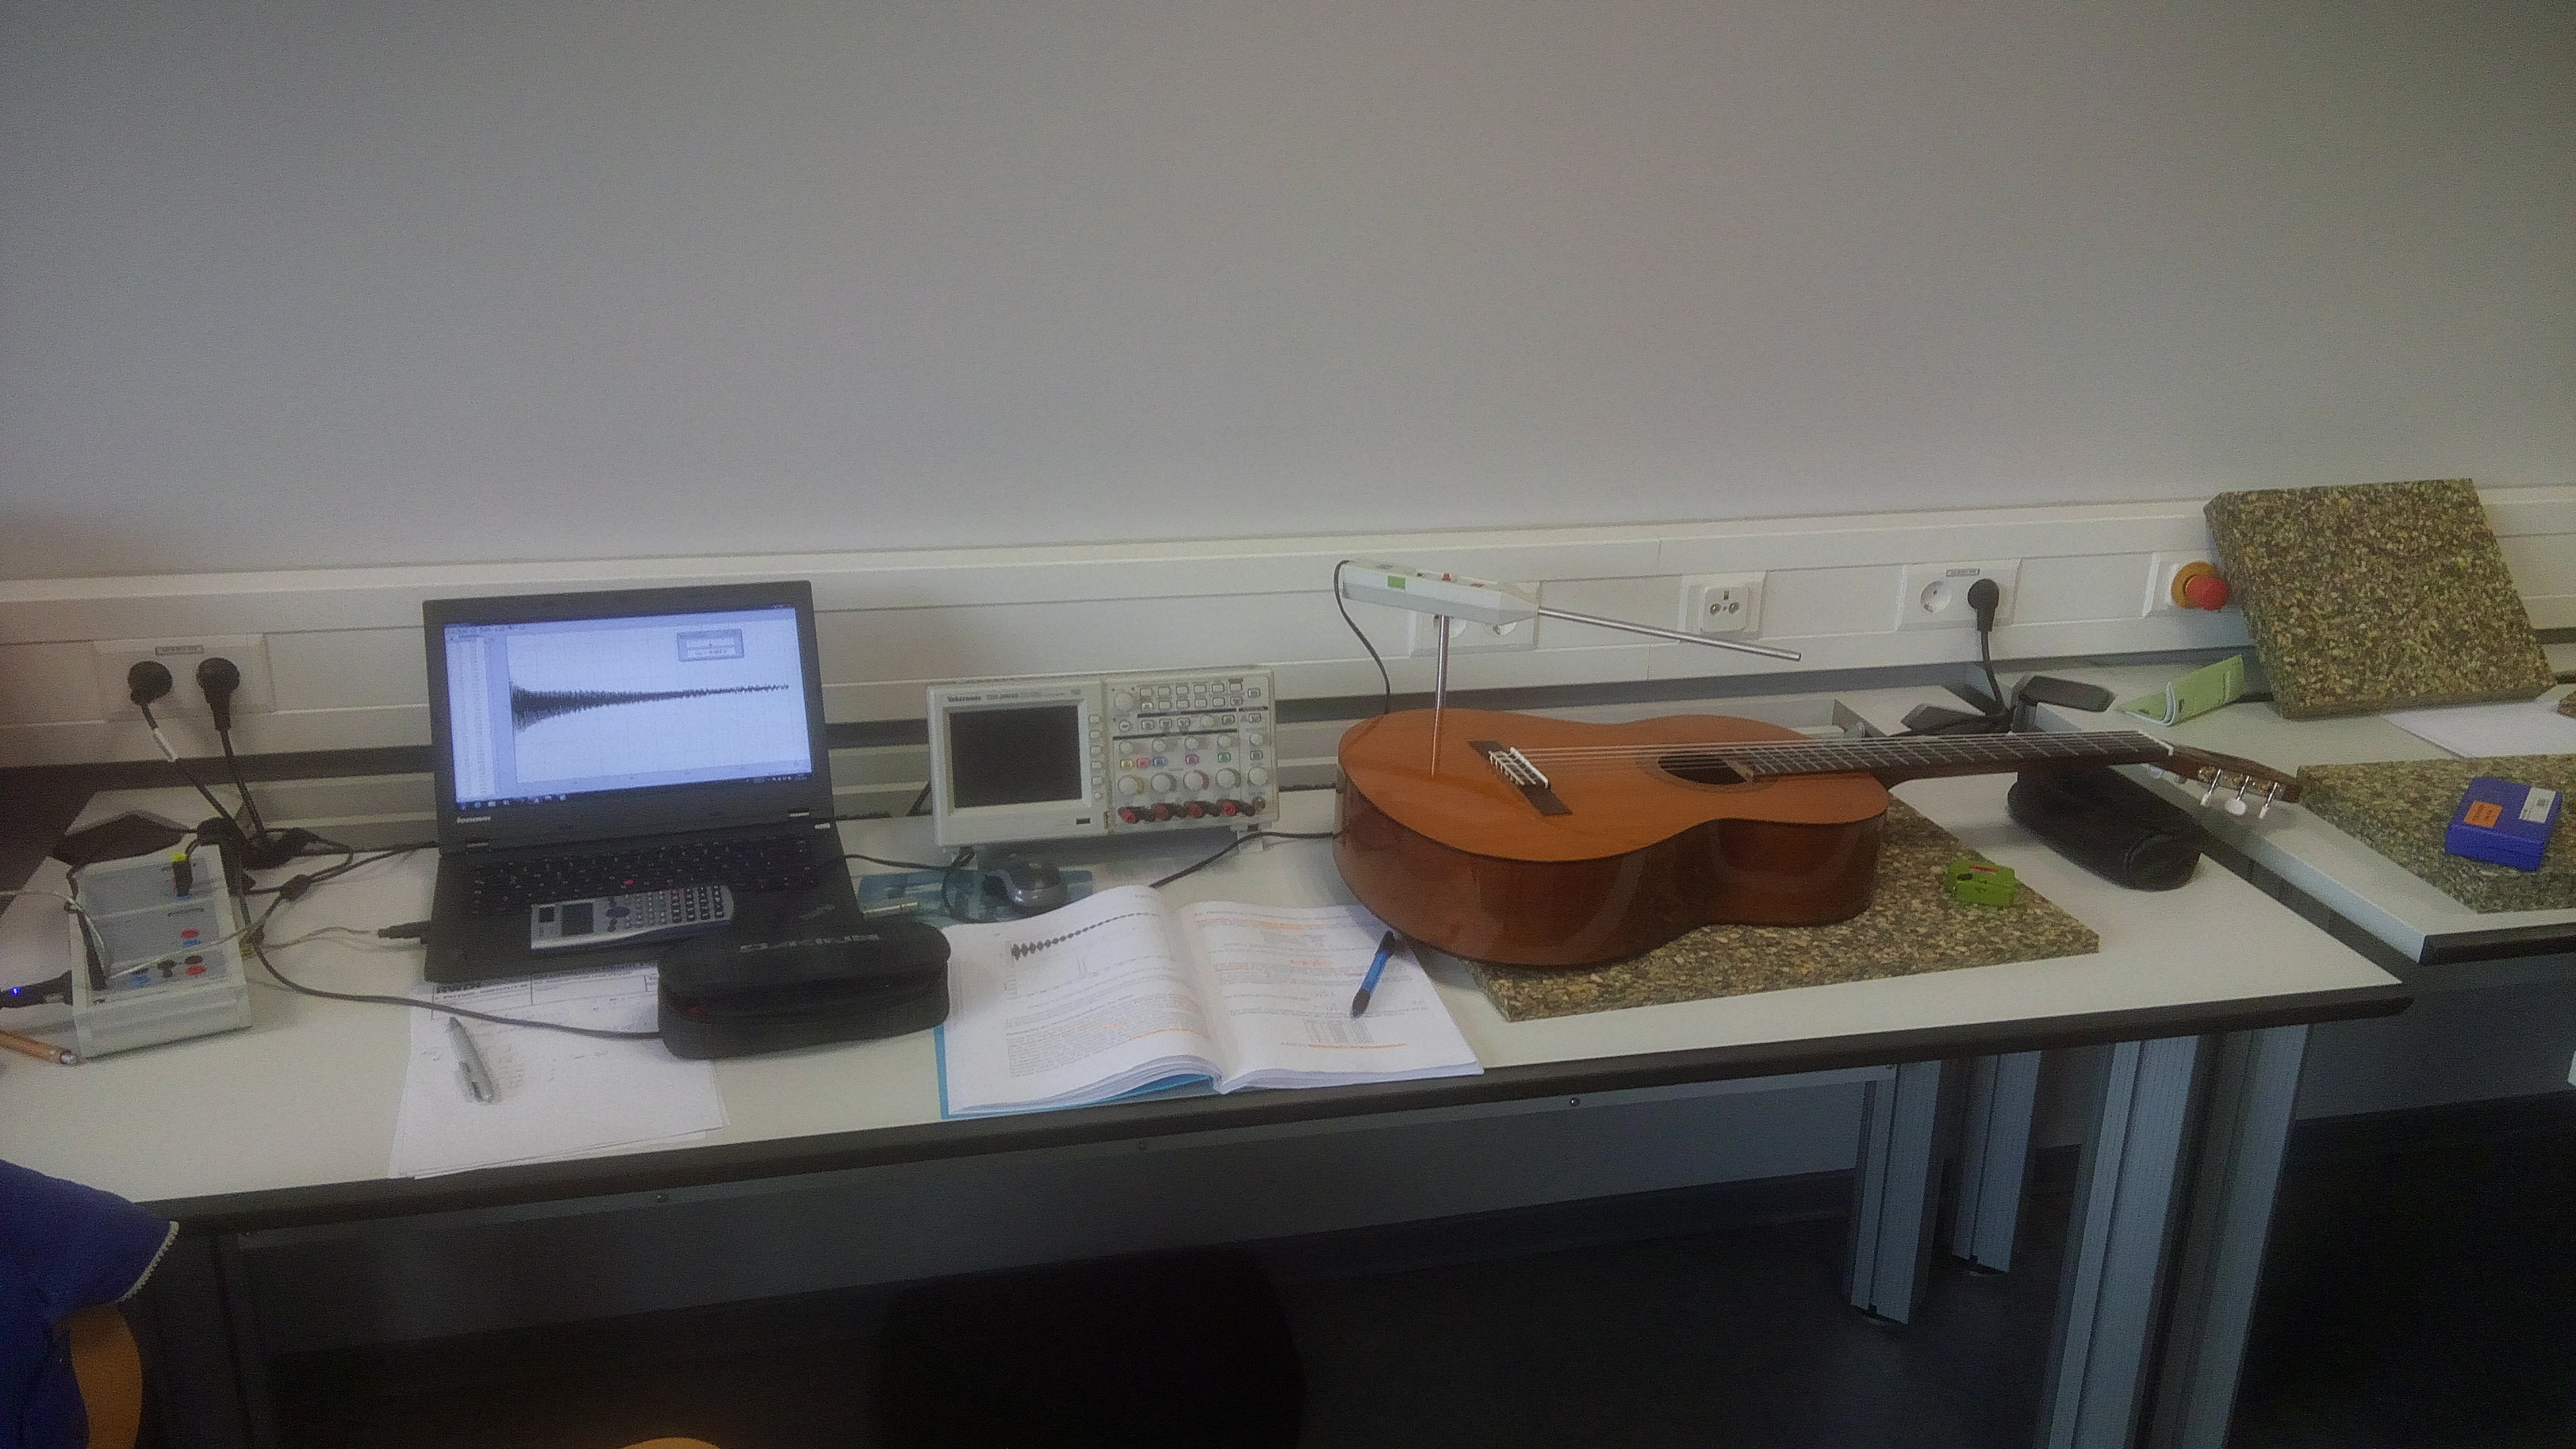
\includegraphics[scale=0.06]{Bilder/IMG_20160323_123920.jpg}
\end{figure}
\end{frame}

\subsection{Erstes Stimmen mit Stimmgerät und Verstimmen}
\begin{frame}
\begin{figure}[H]
\centering
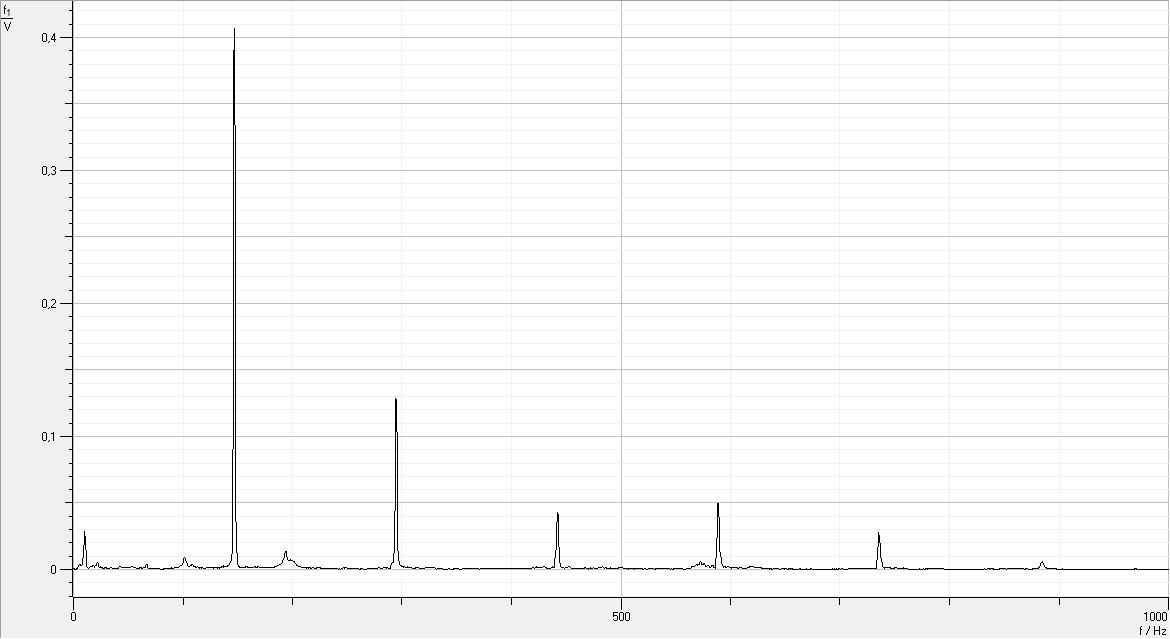
\includegraphics[scale=0.23]{Bilder/Gestimmt_Vorher.png}
\end{figure}
\begin{figure}[H]
\centering
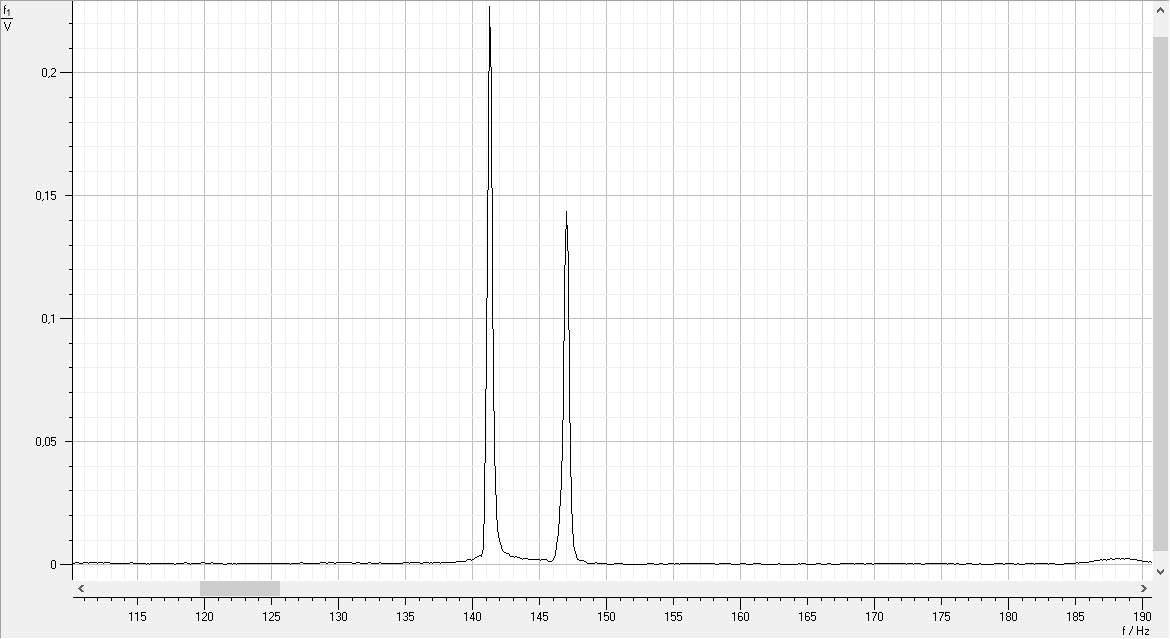
\includegraphics[scale=0.23]{Bilder/Verstimmt.png}
\end{figure}
\end{frame}

\subsection{Stimmversuch 1 und 2}
\begin{frame}
\begin{figure}[H]
\centering
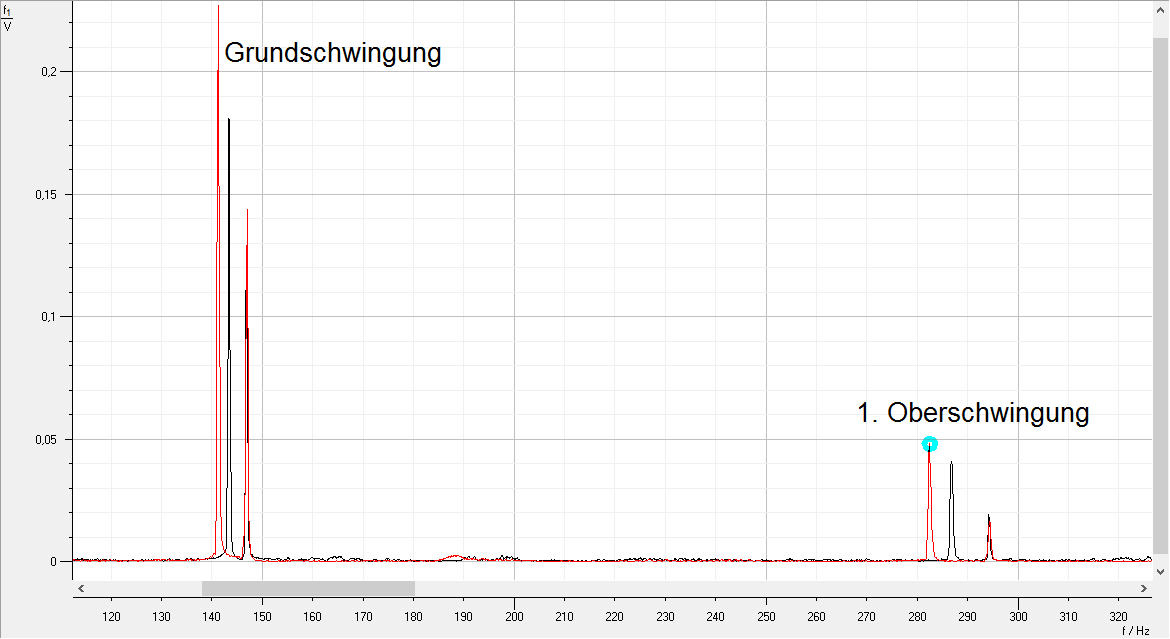
\includegraphics[scale=0.23]{Bilder/Verstimmt_vs_1_stimmen.png}
\end{figure}
\begin{figure}[H]
\centering
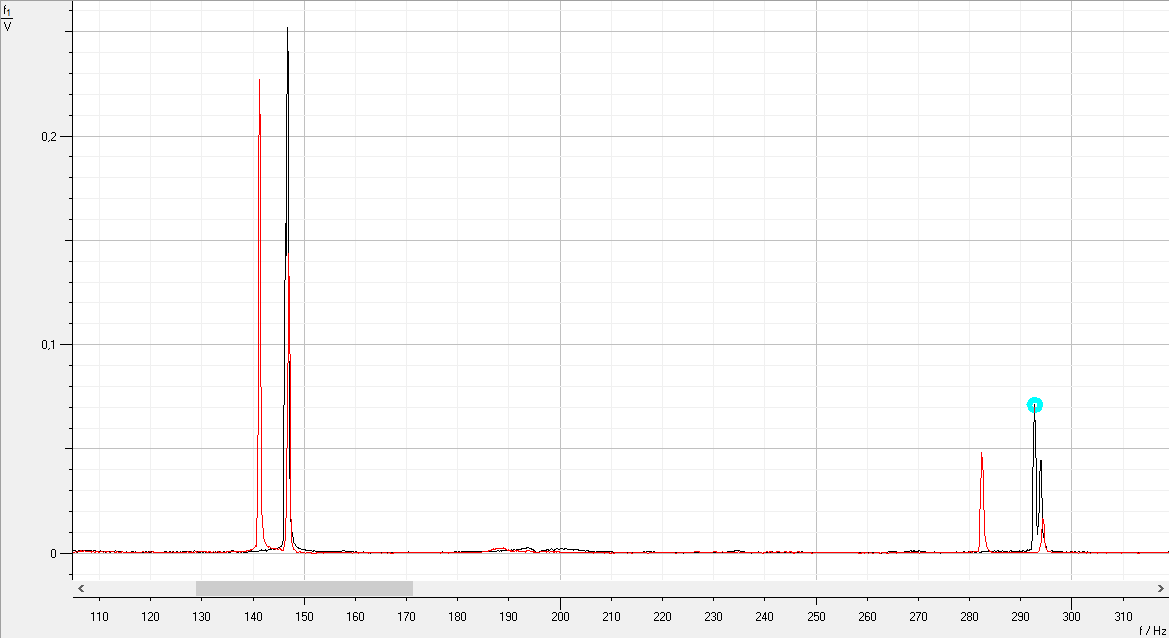
\includegraphics[scale=0.23]{Bilder/Verstimmt_vs_2_stimmen.png}
\end{figure}
\end{frame}

\subsection{3. Stimmversuch}
\begin{frame}
\begin{figure}[H]
\centering
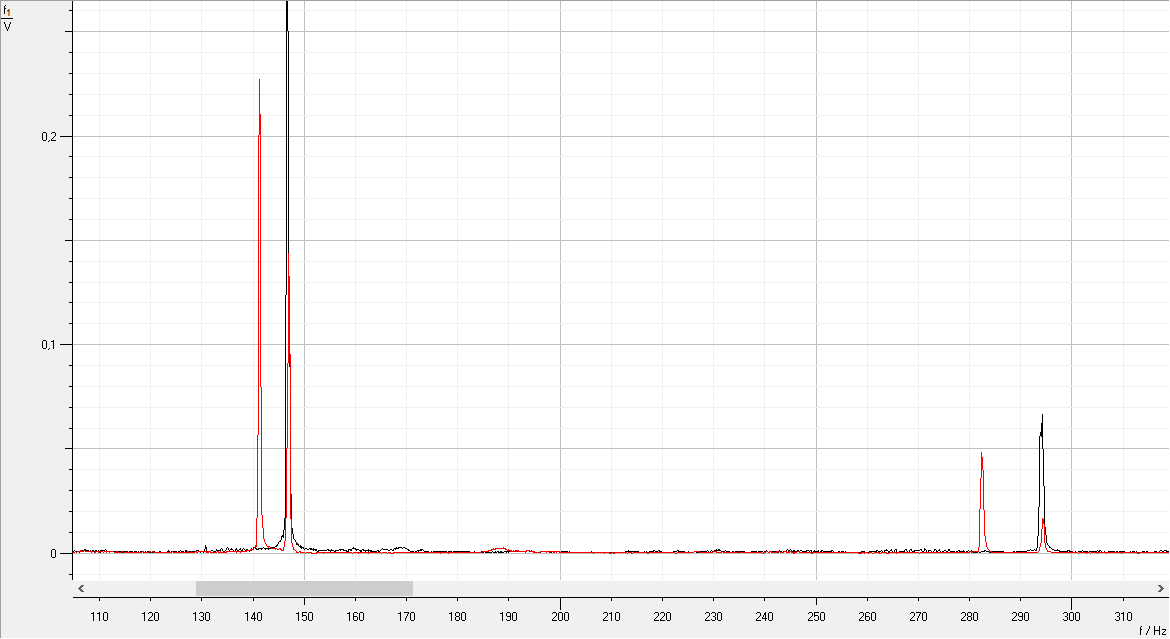
\includegraphics[scale=0.35]{Bilder/Verstimmt_vs_3_stimmen.png}
\end{figure}
\end{frame}

\section{Bestimmung der Materialeigenschaften der Saiten}
\begin{frame}{Bestimmung der Materialeigenschaften der A-Saite}
\begin{equation*}
f=\frac{1}{2}\sqrt{\frac{T}{\mu}}\cdot \frac{1}{l}
\end{equation*}
\begin{equation*}
\mu_{lit}=3.4095 \cdot 10^{-3} \frac{kg}{m}, \hspace{1cm}
T_{lit}=68.04 \text{N.}
\end{equation*}
\begin{equation*}
m_{lit}=\frac{1}{2}\sqrt{\frac{T_{lit}}{\mu_{lit}}}=70.633 \frac{m}{s}
\end{equation*}
\end{frame}

\subsection{Rohdaten}
\begin{frame}
\begin{table}[H]\centering
\begin{tabular}{c|c|c}
$L_0$ & 64.9 cm & Leere Saite\\ 
$L_1$ & 54.6 cm & 2. Bund \\ 
$L_2$ & 51.5 cm & 4. Bund \\ 
$L_3$ & 45.9 cm & 6. Bund \\ 
$L_4$ & 40.9 cm & 8. Bund \\ 
$L_5$ & 36.4 cm & 10. Bund \\ 
\end{tabular} 
\end{table}
\begin{equation*}
\sigma_L=1 mm
\end{equation*}
\begin{table}[H]\centering
\begin{tabular}{c|cccccc}
 & $L_0$ & $L_1$ & $L_2$ & $L_3$ & $L_4$ & $L_5$ \\ 
\hline 
$f_1$ & 110.16 & 123.80 & 138.98 & 156.03 & 174.60 & 194.42 \\ 
$f_2$ & 110.20 & 123.79 & 139.04 & 155.69 & 174.31 & 196.00 \\ 
$f_3$ & 110.24 & 123.79 & 138.83 & 155.96 & 174.46 & 195.97 \\ 
$\bar{f}$ & 110.20 & 123.79 & 138.95 & 155.89 & 174.46 & 195.46 \\ 
$\sigma_{\bar{f}}$ & 0.02 & 0.00 & 0.06  & 0.10 & 0.08  & 0.52  \\ 
\end{tabular}
\newline 
Angaben in Hz
\end{table}
\end{frame}

\subsection{Lineare Regression}
\begin{frame}
\begin{figure}[H]\centering
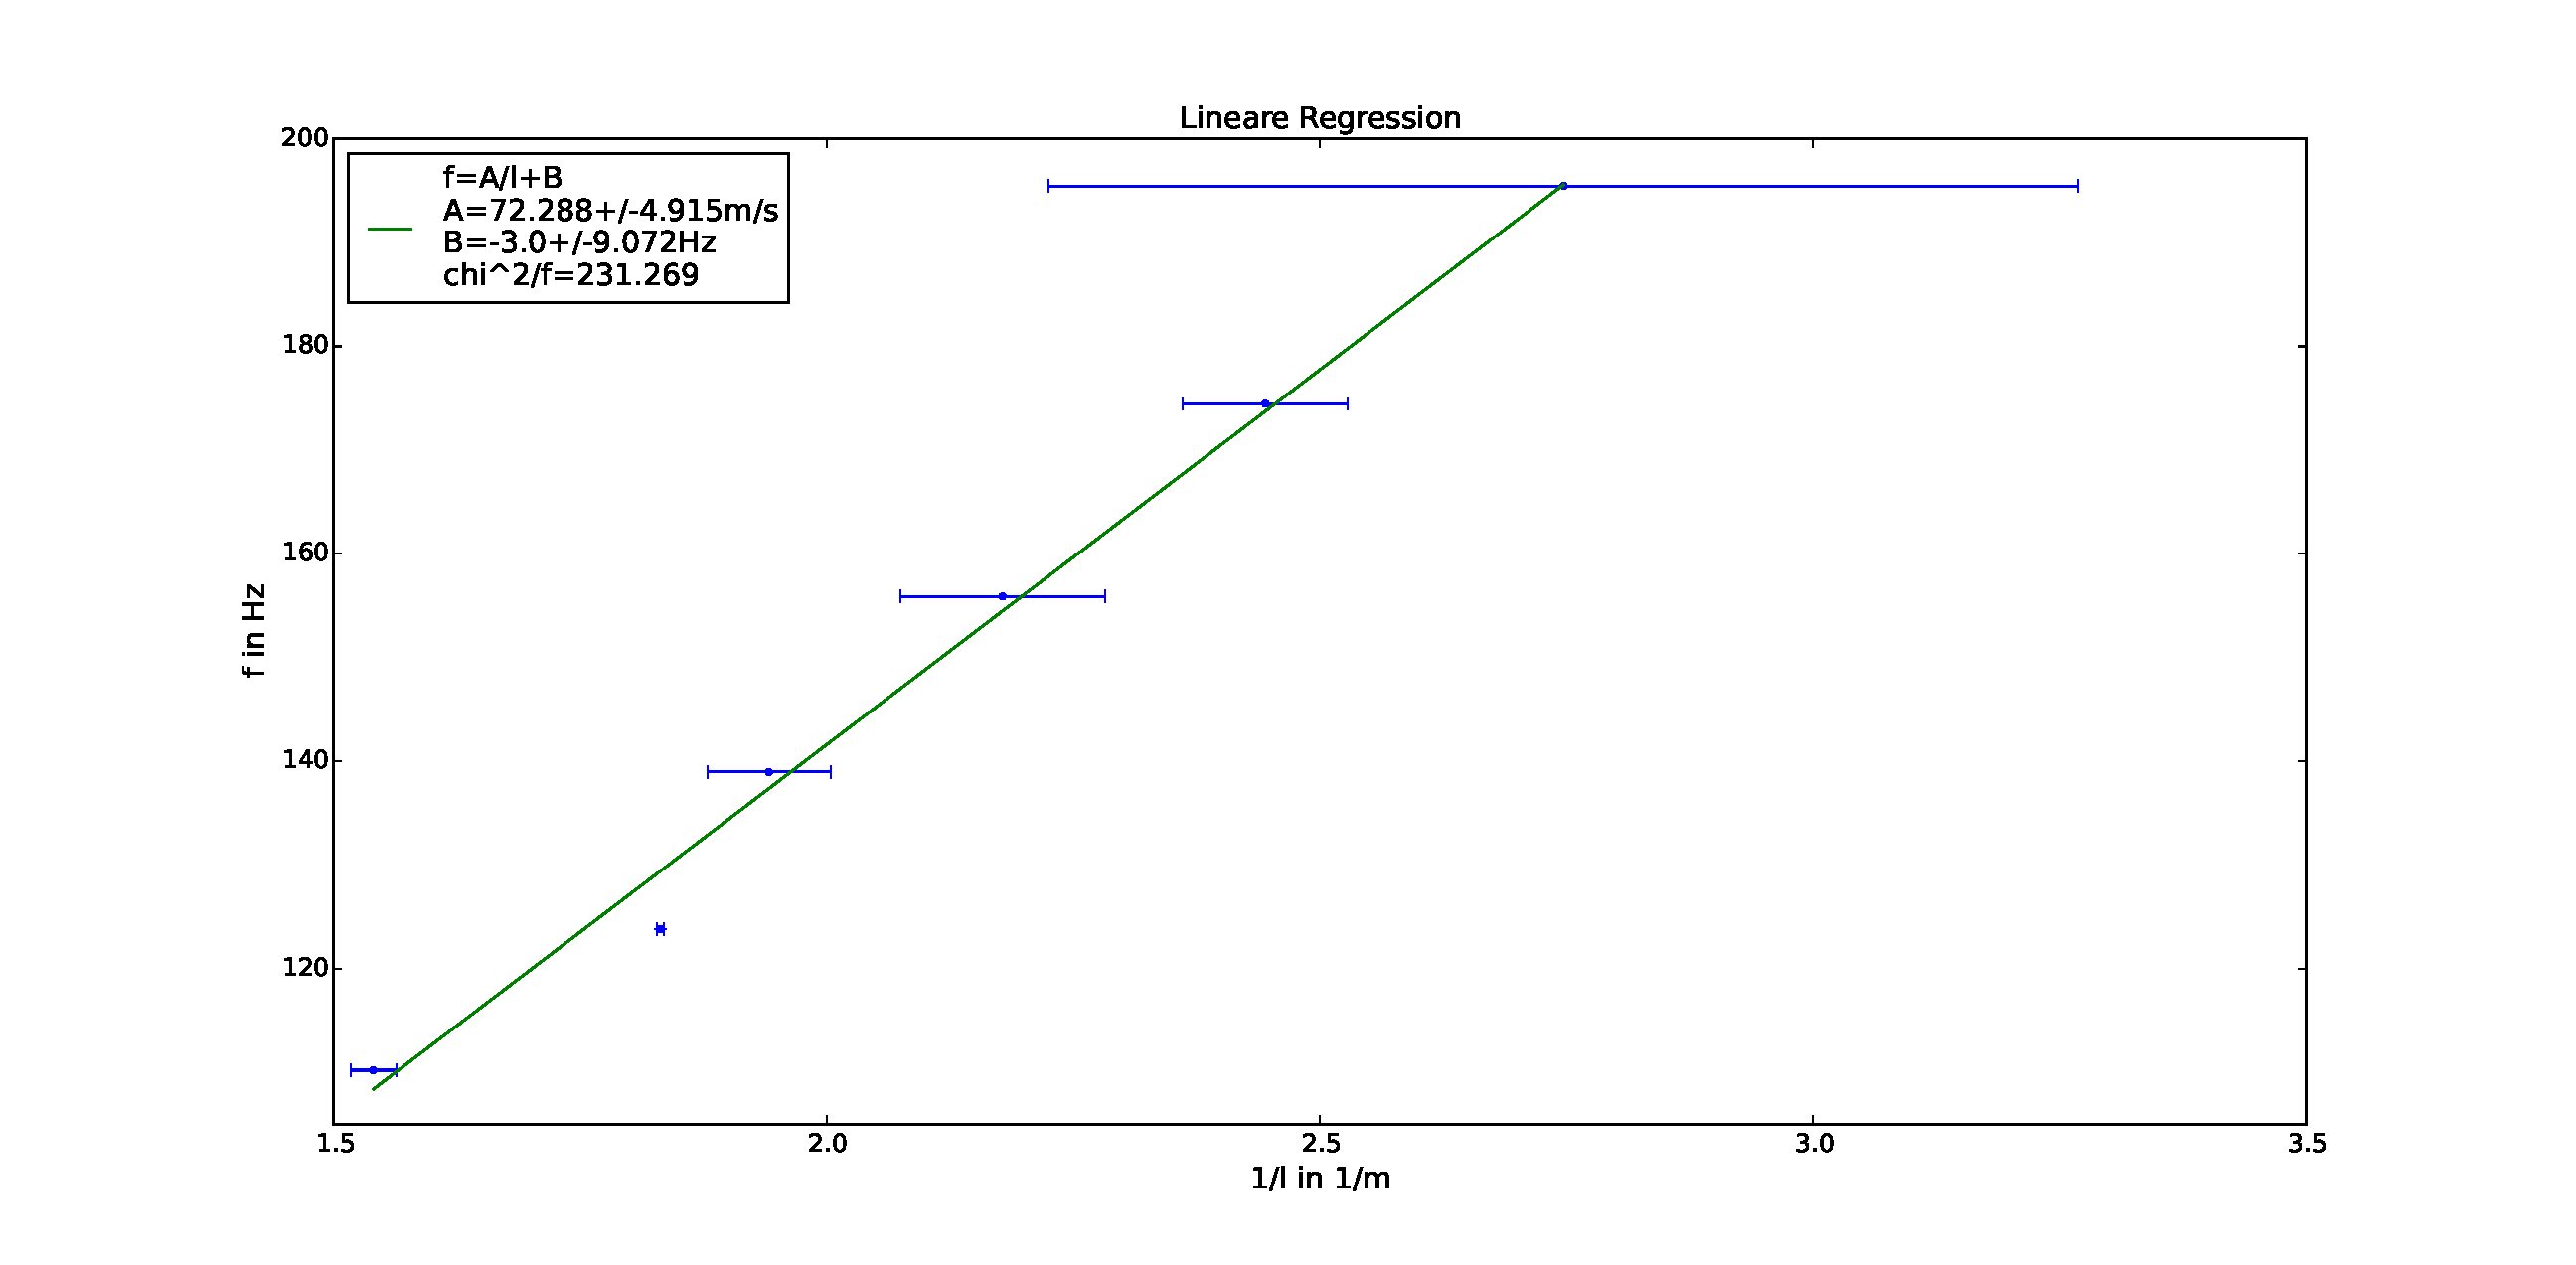
\includegraphics[scale=0.19]{Bilder/lin_reg_mit.eps}
\end{figure}
\begin{figure}[H]
\centering
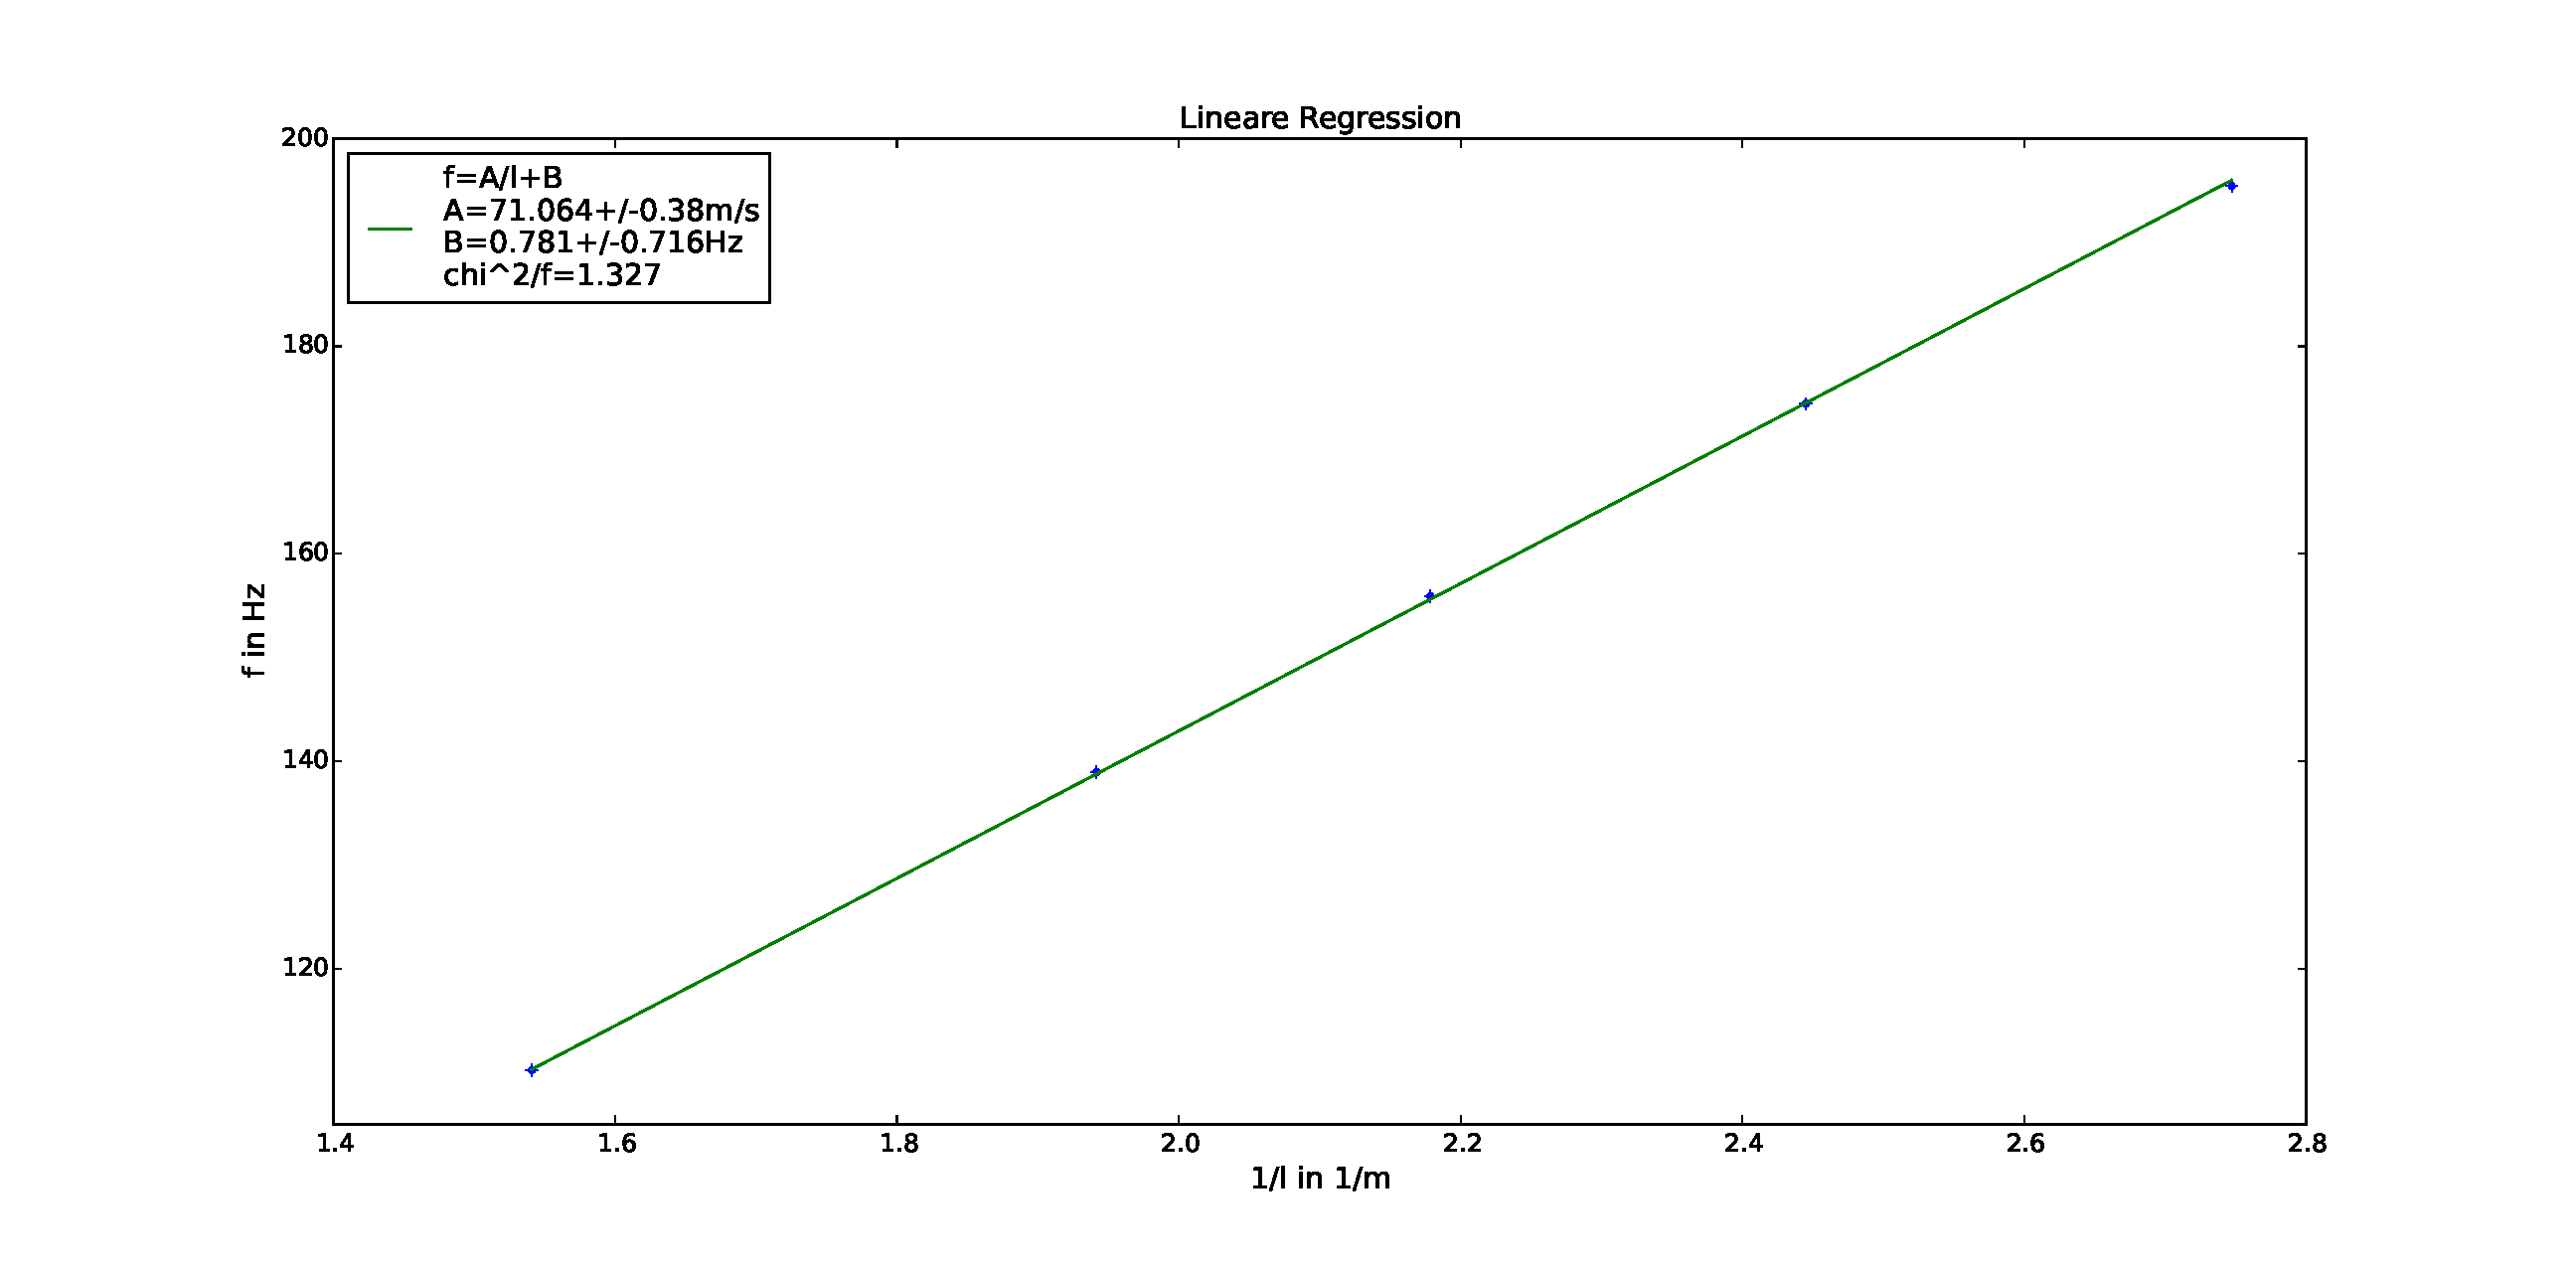
\includegraphics[scale=0.19]{Bilder/lin_reg_ohne.eps}
\end{figure}
\end{frame}

\begin{frame}
\begin{figure}[H]
\centering
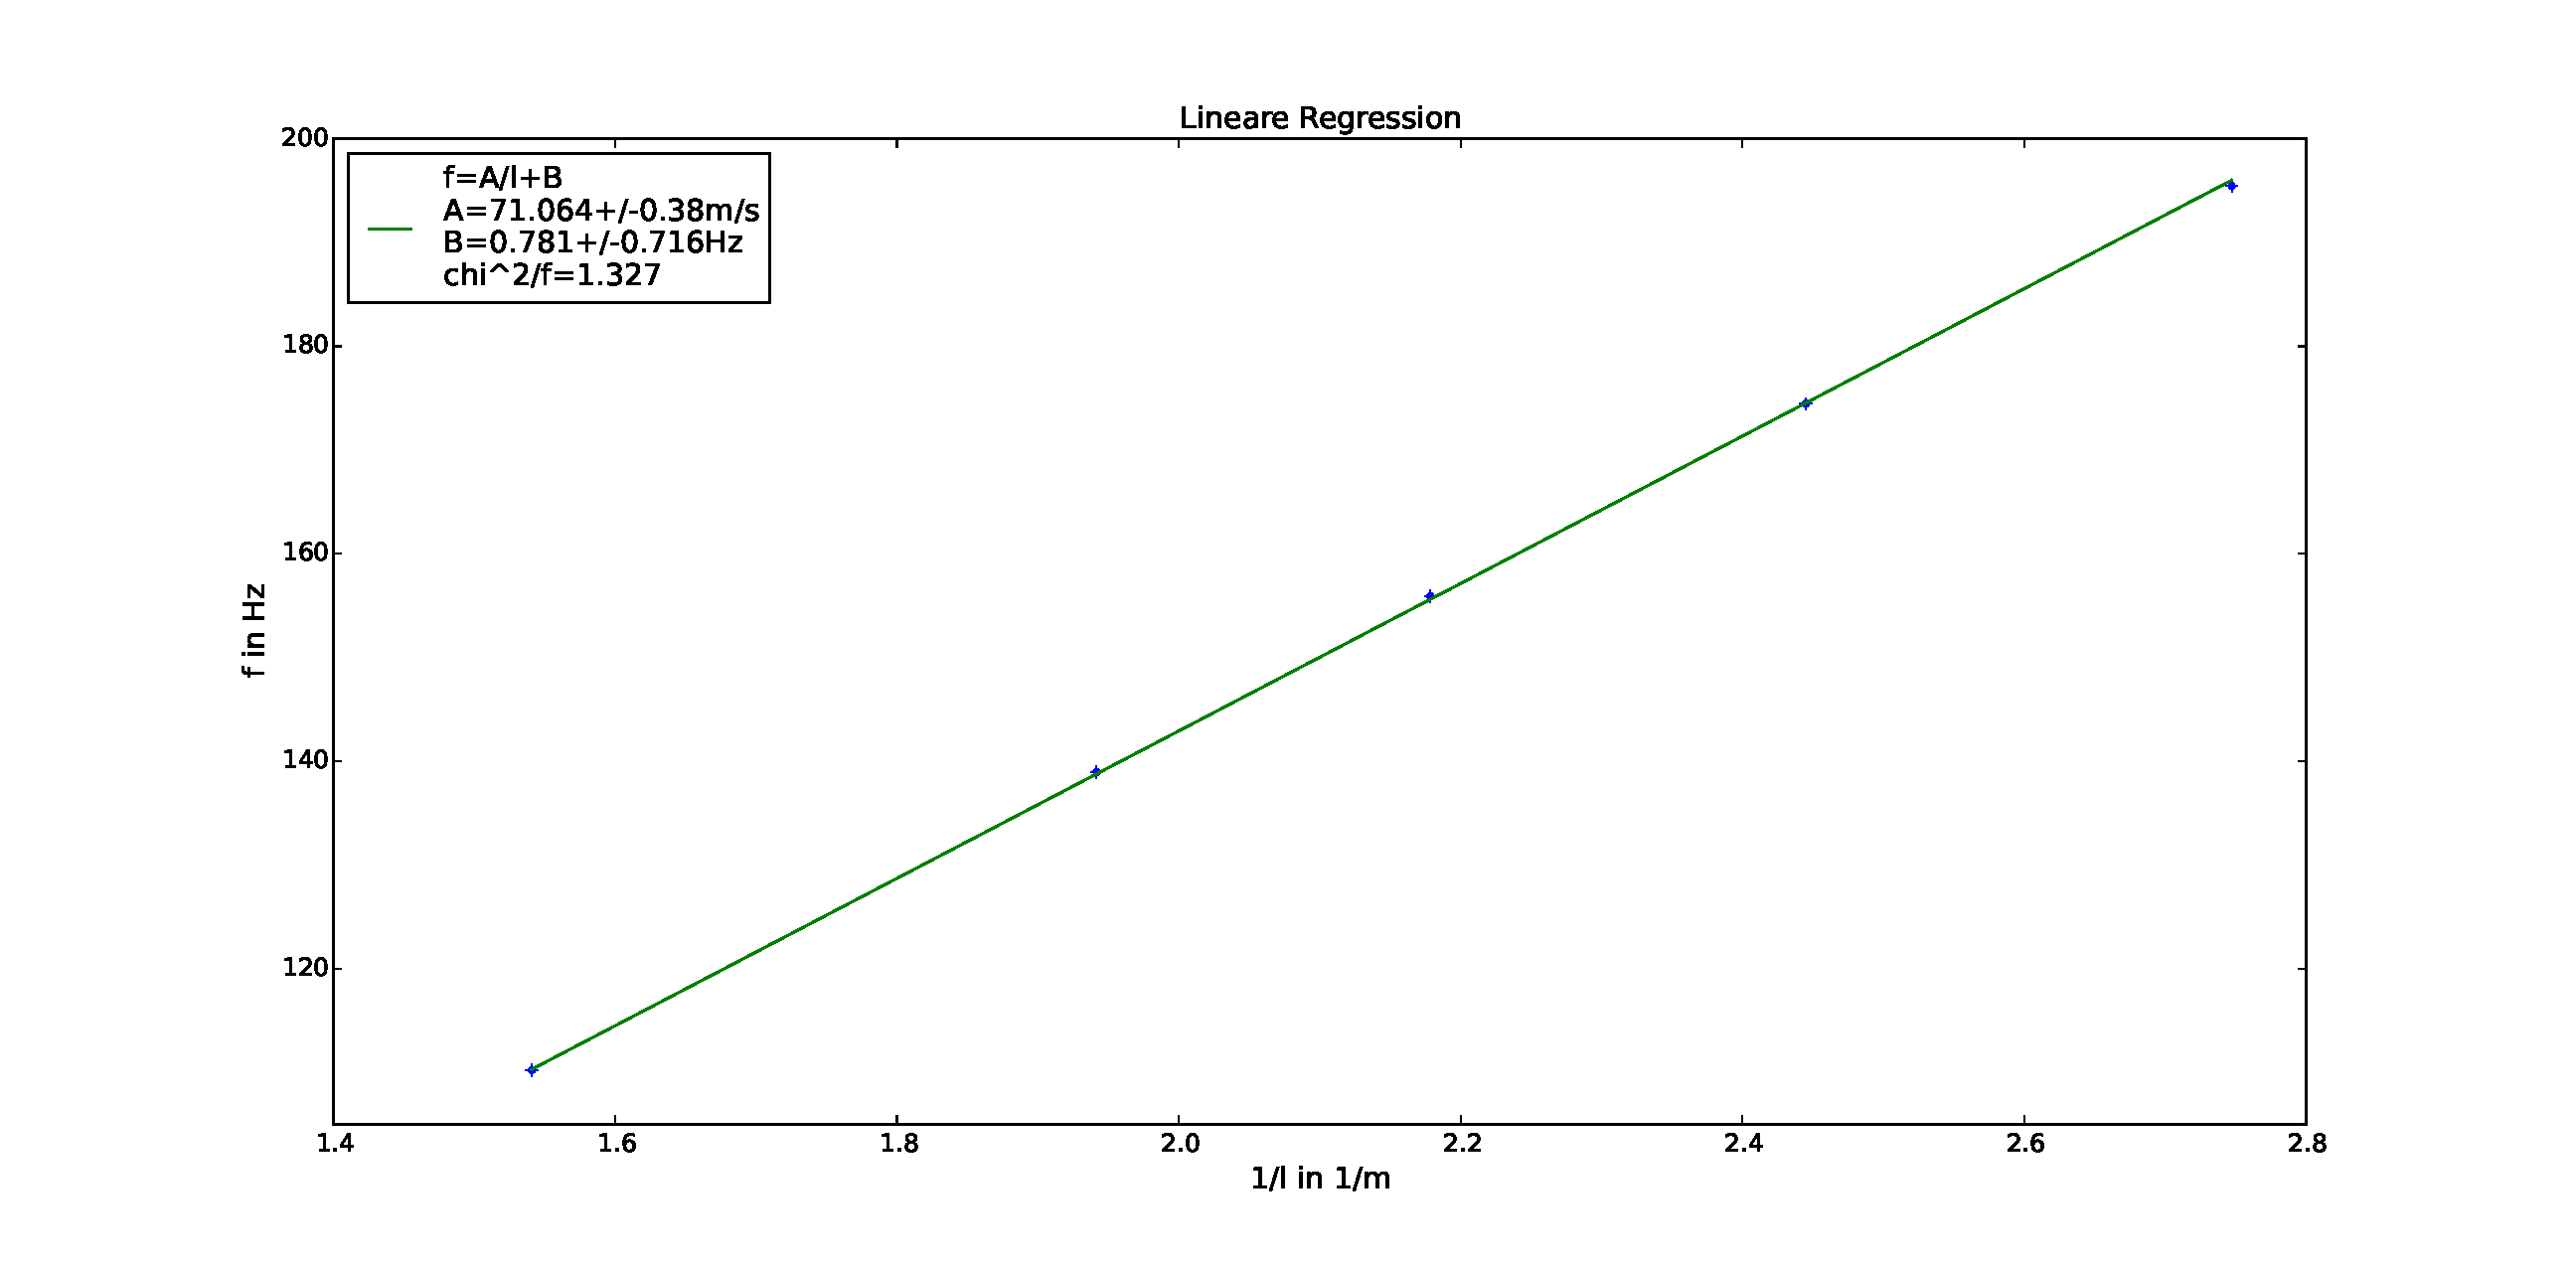
\includegraphics[scale=0.19]{Bilder/lin_reg_ohne.eps}
\end{figure}
\begin{figure}[H]
\centering
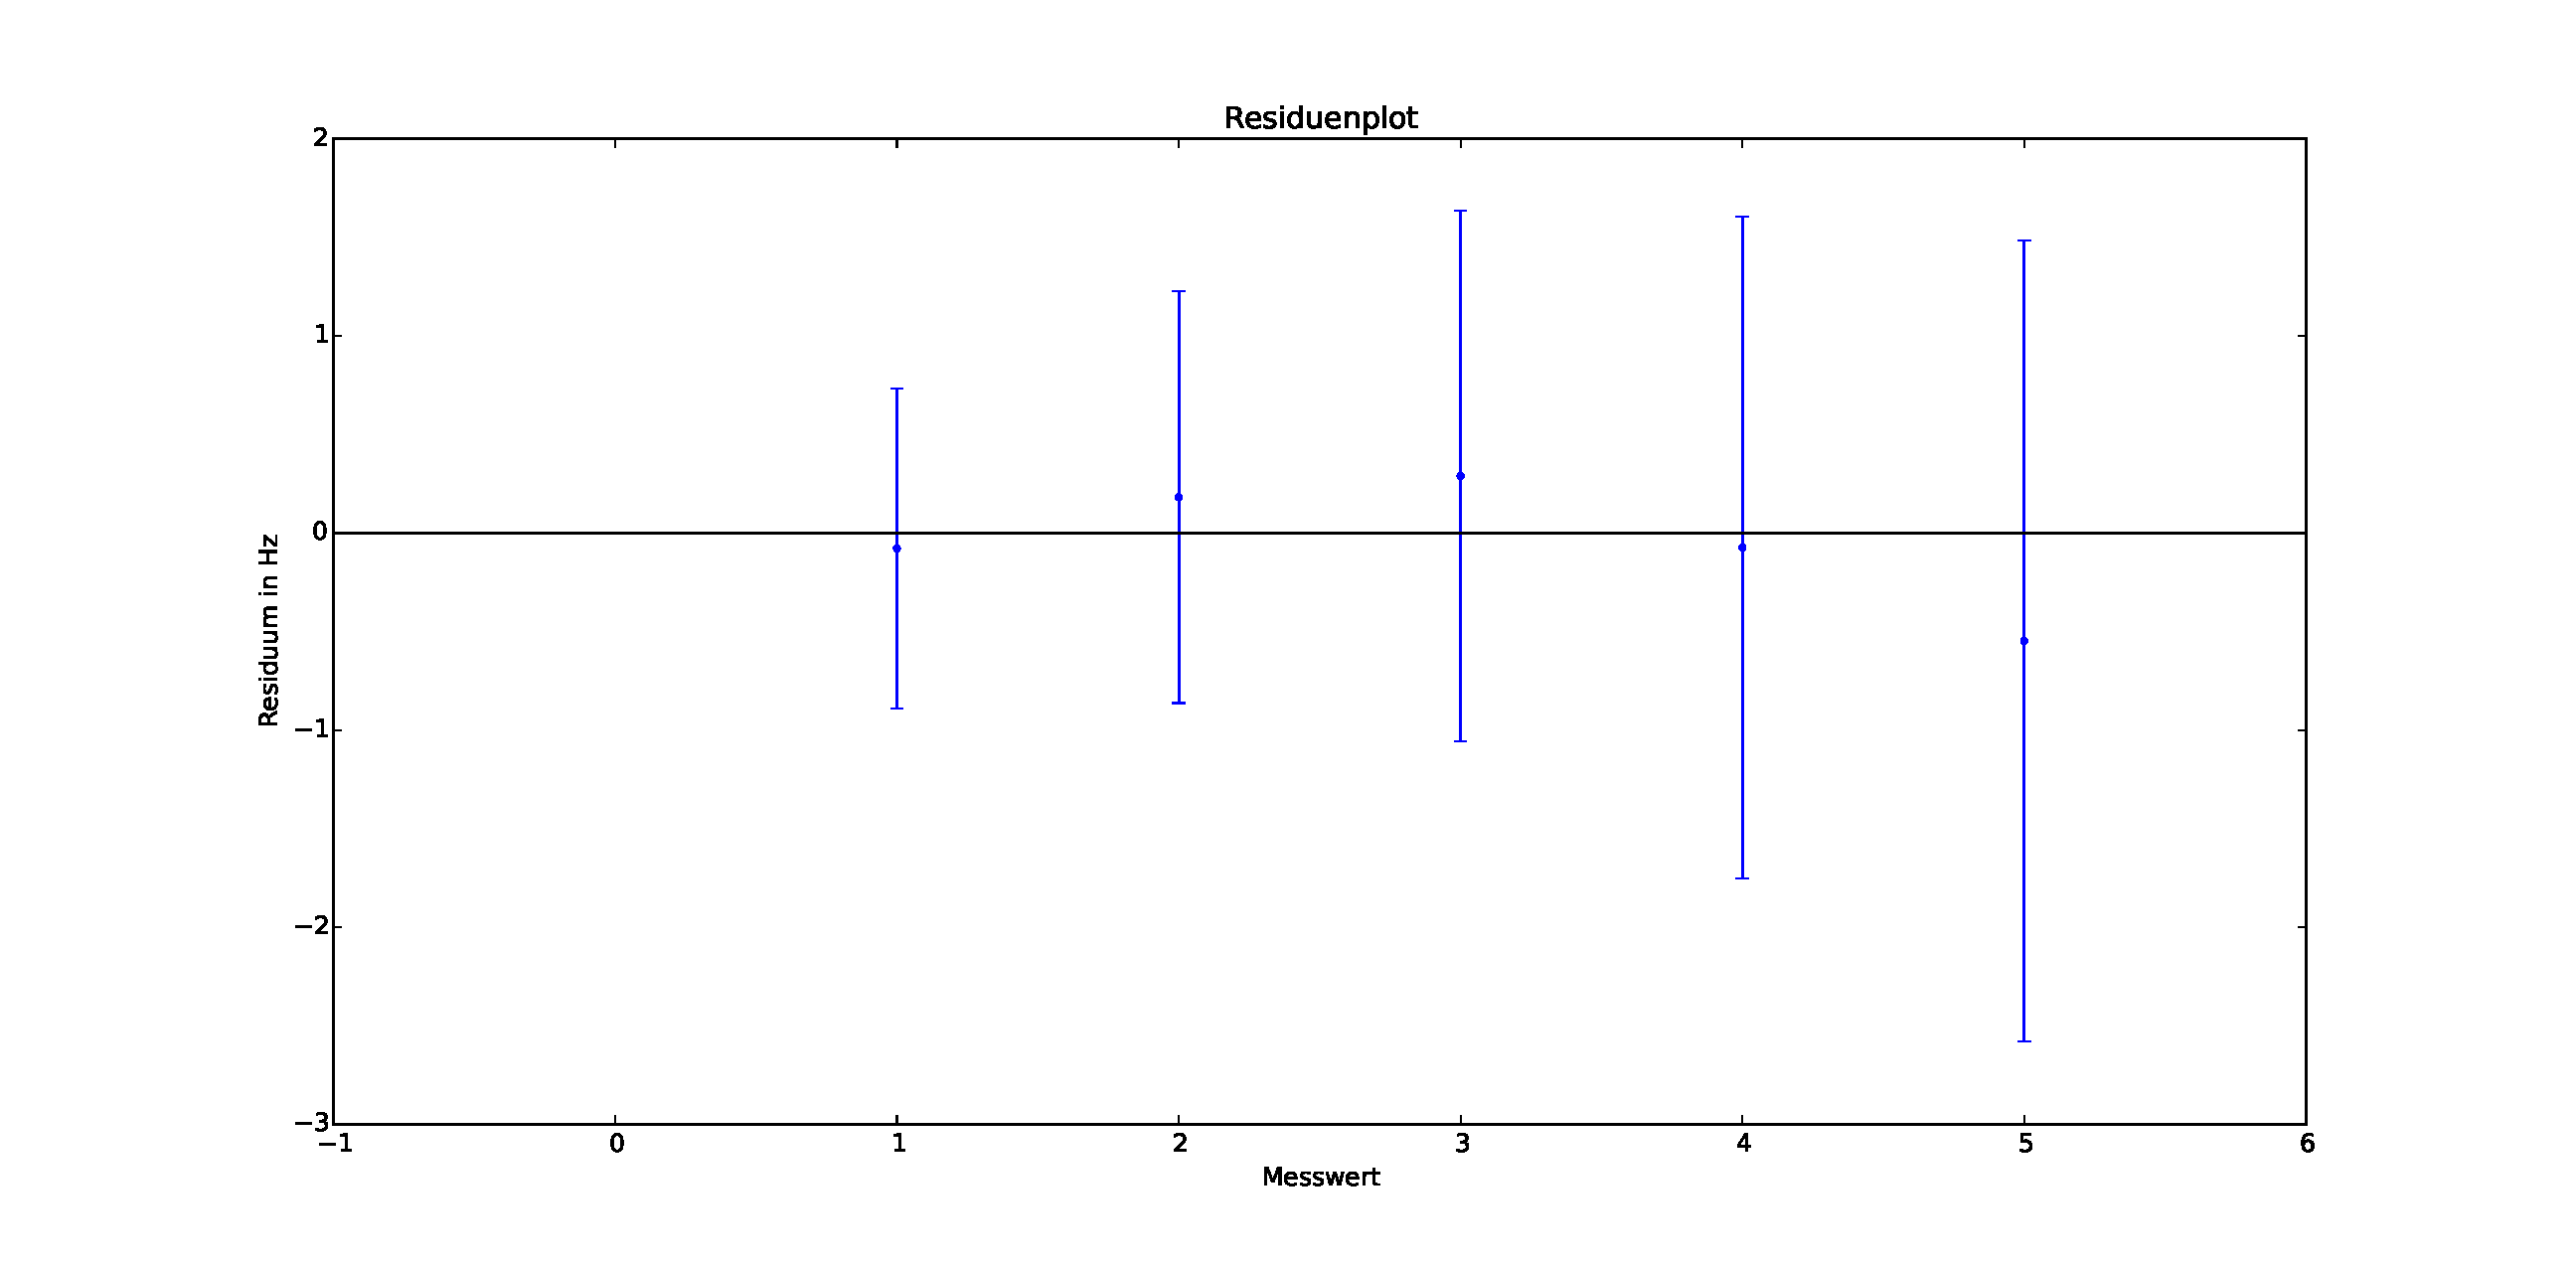
\includegraphics[scale=0.19]{Bilder/lin_reg_ohne_residuum.eps}
\end{figure}
\end{frame}
\subsection{Ergebnis}
\begin{frame}
\begin{align*}
A = m &= 71.162 \pm 0.282 \frac{m}{s}  \\
B &= 0.612 \pm 0.523 Hz \\
\frac{\chi^2}{f}&=0.601
\end{align*}
\begin{equation*}
m_{lit}=70.633 \frac{m}{s}
\end{equation*}
\begin{itemize}
\item innerhalb von 2 $\sigma$ Abweichung
\end{itemize}
\end{frame}

\section{Aufnahme eines Frequenzspektrums}
\begin{frame}{Aufnahme des Frequenzspektrums der D-Saite}
\begin{multicols}{2}
\begin{equation*}
\lambda_n=	\frac{2L}{n}
\end{equation*}
\begin{figure}
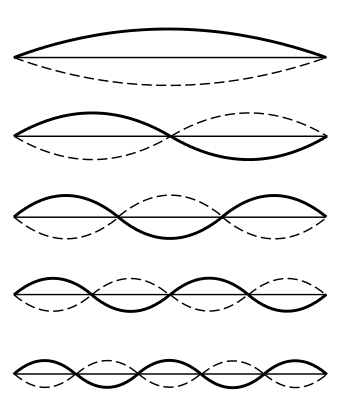
\includegraphics[scale=0.5]{Bilder/Harmonische.png}
\end{figure}
\end{multicols}
\end{frame}
\begin{frame}
\begin{figure}[H]
\centering
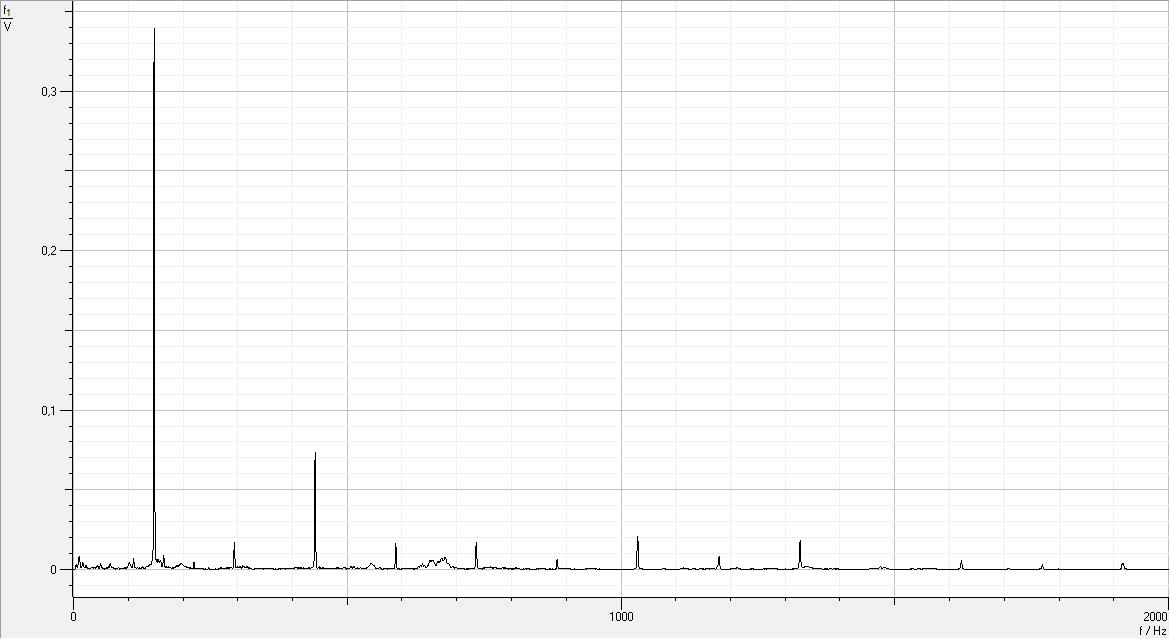
\includegraphics[scale=0.23]{Bilder/Spektrum_Mitte.png}

\end{figure}

\begin{figure}[H]
\centering
\includegraphics[scale=0.23]{Bilder/Spektrum_oben.png}
\end{figure}
\end{frame}

\section{Fazit}
\begin{frame}
\begin{itemize}
\item Schallgeschwindigkeiten in 1. und 3. Stange passten nicht gut.
\item Schallgeschwindigkeiten in 2. und 4. Stange passten gut.
\item Die D-Saite konnte durch Schwebung erfolgreich gestimmt werden.
\item Die Materialkonstante der A-Saite stimmt mit etwas mehr als 1$\sigma$ mit dem Literaturwert überein.
\item n-te Harmonische fehlt, wenn die Saite bei $d=\frac{L}{n}$ angeschlagen wird.
\end{itemize}
\end{frame}


\end{document}